\documentclass{beamer}
\usepackage{amsmath}
\usepackage[english]{babel} %set language; note: after changing this, you need to delete all auxiliary files to recompile
\usepackage[utf8]{inputenc} %define file encoding; latin1 is the other often used option
\usepackage{csquotes} % provides context sensitive quotation facilities
\usepackage{graphicx} %allows for inserting figures
\usepackage{booktabs} % for table formatting without vertical lines
\usepackage{textcomp} % allow for example using the Euro sign with \texteuro
\usepackage{stackengine}
\usepackage{wasysym}
\usepackage{tikzsymbols}
\usepackage{textcomp}
\newcommand{\bubblethis}[2]{
        \tikz[remember picture,baseline]{\node[anchor=base,inner sep=0,outer sep=0]%
        (#1) {\underline{#1}};\node[overlay,cloud callout,callout relative pointer={(0.2cm,-0.7cm)},%
        aspect=2.5,fill=yellow!90] at ($(#1.north)+(-0.5cm,1.6cm)$) {#2};}%
    }%
\tikzset{face/.style={shape=circle,minimum size=4ex,shading=radial,outer sep=0pt,
        inner color=white!50!yellow,outer color= yellow!70!orange}}
%% Some commands to make the code easier
\newcommand{\emoticon}[1][]{%
  \node[face,#1] (emoticon) {};
  %% The eyes are fixed.
  \draw[fill=white] (-1ex,0ex) ..controls (-0.5ex,0.2ex)and(0.5ex,0.2ex)..
        (1ex,0.0ex) ..controls ( 1.5ex,1.5ex)and( 0.2ex,1.7ex)..
        (0ex,0.4ex) ..controls (-0.2ex,1.7ex)and(-1.5ex,1.5ex)..
        (-1ex,0ex)--cycle;}
\newcommand{\pupils}{
  %% standard pupils
  \fill[shift={(0.5ex,0.5ex)},rotate=80] 
       (0,0) ellipse (0.3ex and 0.15ex);
  \fill[shift={(-0.5ex,0.5ex)},rotate=100] 
       (0,0) ellipse (0.3ex and 0.15ex);}

\newcommand{\emoticonname}[1]{
  \node[below=1ex of emoticon,font=\footnotesize,
        minimum width=4cm]{#1};}
\usepackage{scalerel}
\usetikzlibrary{positioning}
\usepackage{xcolor,amssymb}
\newcommand\dangersignb[1][2ex]{%
  \scaleto{\stackengine{0.3pt}{\scalebox{1.1}[.9]{%
  \color{red}$\blacktriangle$}}{\tiny\bfseries !}{O}{c}{F}{F}{L}}{#1}%
}
\newcommand\dangersignw[1][2ex]{%
  \scaleto{\stackengine{0.3pt}{\scalebox{1.1}[.9]{%
  \color{red}$\blacktriangle$}}{\color{white}\tiny\bfseries !}{O}{c}{F}{F}{L}}{#1}%
}
\usepackage{fontawesome} % Social Icons
\usepackage{epstopdf} % allow embedding eps-figures
\usepackage{tikz} % allows drawing figures
\usepackage{amsmath,amssymb,amsthm} %advanced math facilities
\usepackage{lmodern} %uses font that support italic and bold at the same time
\usepackage{hyperref}
\usepackage{tikz}
\hypersetup{
    colorlinks=true,
    linkcolor=blue,
    filecolor=magenta,      
    urlcolor=blue,
}
\usepackage{tcolorbox}
%add citation management using BibLaTeX
\usepackage[citestyle=authoryear-comp, %define style for citations
    bibstyle=authoryear-comp, %define style for bibliography
    maxbibnames=10, %maximum number of authors displayed in bibliography
    minbibnames=1, %minimum number of authors displayed in bibliography
    maxcitenames=3, %maximum number of authors displayed in citations before using et al.
    minnames=1, %maximum number of authors displayed in citations before using et al.
    datezeros=false, % do not print dates with leading zeros
    date=long, %use long formats for dates
    isbn=false,% show no ISBNs in bibliography (applies only if not a mandatory field)
    url=false,% show no urls in bibliography (applies only if not a mandatory field)
    doi=false, % show no dois in bibliography (applies only if not a mandatory field)
    eprint=false, %show no eprint-field in bibliography (applies only if not a mandatory field)
    backend=biber %use biber as the backend; backend=bibtex is less powerful, but easier to install
    ]{biblatex}
\addbibresource{../mybibfile.bib} %define bib-file located one folder higher


\usefonttheme[onlymath]{serif} %set math font to serif ones

\definecolor{beamerblue}{rgb}{0.2,0.2,0.7} %define beamerblue color for later use

%%% defines highlight command to set text blue
\newcommand{\highlight}[1]{{\color{blue}{#1}}}


%%%%%%% commands defining backup slides so that frame numbering is correct

\newcommand{\backupbegin}{
   \newcounter{framenumberappendix}
   \setcounter{framenumberappendix}{\value{framenumber}}
}
\newcommand{\backupend}{
   \addtocounter{framenumberappendix}{-\value{framenumber}}
   \addtocounter{framenumber}{\value{framenumberappendix}}
}

%%%% end of defining backup slides

%Specify figure caption, see also http://tex.stackexchange.com/questions/155738/caption-package-not-working-with-beamer
\setbeamertemplate{caption}{\insertcaption} %redefines caption to remove label "Figure".
%\setbeamerfont{caption}{size=\scriptsize,shape=\itshape,series=\bfseries} %sets figure  caption bold and italic and makes it smaller


\usetheme{Boadilla}

%set options of hyperref package
\hypersetup{
    bookmarksnumbered=true, %put section numbers in bookmarks
    naturalnames=true, %use LATEX-computed names for links
    citebordercolor={1 1 1}, %color of border around cites, here: white, i.e. invisible
    linkbordercolor={1 1 1}, %color of border around links, here: white, i.e. invisible
    colorlinks=true, %color links
    anchorcolor=black, %set color of anchors
    linkcolor=beamerblue, %set link color to beamer blue
    citecolor=blue, %set cite color to beamer blue
    pdfpagemode=UseThumbs, %set default mode of PDF display
    breaklinks=true, %break long links
    pdfstartpage=1 %start at first page
    }


% --------------------
% Overall information
% --------------------
\title[Principios de Economía]{Principios de Economía}
\date{}
\author[Ertola y Sturzenegger]{Gabriela Ertola y Federico Sturzenegger }
\vspace{0.4cm}
\institute[]{Universidad de San Andrés \\
2022} 


\begin{document}

\begin{frame}
\frametitle{Principios de Economía
\centering
\\ \vspace{12mm} Interacciones sociales}
\centering
 \\ \vspace{12mm} %5 de agosto, 2021 \vspace{5mm} \\ 

\includegraphics[scale=0.25]{Figures/logoUDESA.jpg} 
\end{frame}


\begin{frame}
\frametitle{¿Qué sucede cuando interactuamos con otros?}
\begin{itemize}
    \item En los modelos que vimos hasta ahora, las decisiones de los individuos no dependían de las decisiones de otros
    \item Pero, la verdad es que solemos interactuar con otros seres humanos!
    \item La interacción genera distintos tipos de consecuencias, que afectan las decisiones de los demás individuos
    \item ¿De qué modo la interacción afecta a los individuos? 
\end{itemize} 
\end{frame}

\begin{frame}
\frametitle{Especialización}
    \begin{itemize}
    \item ¿Conocen la historia de Robinson Crusoe?
    \item ¿Qué sucede cuando aparece Viernes?  
    \end{itemize}
    \centering \vspace{3mm}
    \begin{tabular}{|c|c|c|} \hline
        & Robinson Crusoe & Viernes \\ \hline
     Pescados   & 4 & 3 \\ \hline
     Cocos   & 6 & 2 \\ \hline     \end{tabular}
    \begin{itemize}
    \item ¿Qué sucede si quieren consumir 6 pescados y 6 cocos por día? 
    \item ¿Les conviene especializarse?  
    \end{itemize}
\end{frame}

\begin{frame}
\frametitle{Especialización}
\begin{itemize}
    \item Costo de oportunidad de Robinson...
        \begin{itemize}
        \item de pescar en vez de recolectar cocos: $ 6/4 = 1,5 $ cocos por pescado 
        \item de recolectar cocos en vez de pescar: $ 4/6 = 2/3=0,66 $ pescados por coco
        \end{itemize}
    \item Costo de oportunidad de Viernes...
        \begin{itemize}
        \item de pescar en vez de recolectar cocos: $ 2/3 = 0,66 $ cocos por pescado
        \item de recolectar cocos en vez de pescar: $ 3/2 = 1,5 $ pescados por coco
        \end{itemize}
    \item Para ver las ventajas del comercio y la especialización debemos comparar los costos de oportunidad de los bienes entre los individuos
\end{itemize}
\end{frame}

\begin{frame}
\frametitle{ Especialización}
\begin{itemize}
    \item Costo de oportunidad de pescar en vez de recolectar cocos:
        \begin{itemize}
        \item Viernes: $ 2/3 < 1,5 $ Robinson 
        \end{itemize}
    \item Costo de oportunidad de recolectar cocos en vez de pescar:
        \begin{itemize}
        \item Viernes: $ 1,5 > 2/3 $ Robinson 
        \end{itemize}
    \item Si se especializan ahora Robinson debe trabajar media hora menos y Viernes 1 hora menos que en el caso de no especialización. 
\end{itemize}
\end{frame}

\begin{frame}
\frametitle{ Especialización}
\begin{itemize}
    \item La división del trabajo (o especialización), permite aumentar la producción... ¿por qué?  
    \begin{itemize}
        \item Learning-by-doing \\
        Desarrollo de habilidades cuando se produce algo 
        \item Economías de escala\\
        Producir en grandes cantidades suele ser más costo-efectivo
        \item Heterogeneidad y ventaja comparativa \\
        Agentes difieren en habilidades o recursos, lo que los hace más o menos productivos en una actividad particular
    \end{itemize}
\end{itemize} 
\end{frame}

\begin{frame}
\frametitle{ Un modelo Ricardiano simple}
\begin{itemize}
    \item 2 países: Inglaterra y Portugal
    \item Dos productos: vino y telas
    \item Portugal tiene la ventaja absoluta en ambos. \\
    Inglaterra puede producirlos, pero Portugal tiene condiciones favorables tanto para producir uvas (para hacer el vino), como para criar ovejas (que dan la lana para las telas)
    \item Para Inglaterra es relativamente más difícil producir vino
    \item Inglaterra tendrá una ventaja comparativa en la tela y se la exportará a Portugal
\end{itemize} 
\end{frame}

\begin{frame}
\frametitle{ Un modelo Ricardiano simple}
\begin{itemize}
    \item Supongamos que en Portugal (P) e Inglaterra (I) los bienes se producen sólo con trabajo (L), los trabajadores de cada país son:
    \begin{itemize}
        \item $L_P=25$
        \item $L_I=100$
    \end{itemize}
    \item La productividad marginal del trabajo... \begin{itemize}
        \item ... en Portugal un trabajador puede producir 4 botellas de vino o 2 metros de tela \\
        $PMgL_V = 4$ y $PMgL_t = 2$
        \item ... en Inglaterra un trabajador puede producir 1 botella de vino o 1 metro de tela \\
        $PMgLv = 1$ y $PMgLt = 1$
        \end{itemize} 
    \item ¿Cuáles son las posibilidades de producción?    
\end{itemize} 
\end{frame}

\begin{frame}
\frametitle{ Portugal}
\centering
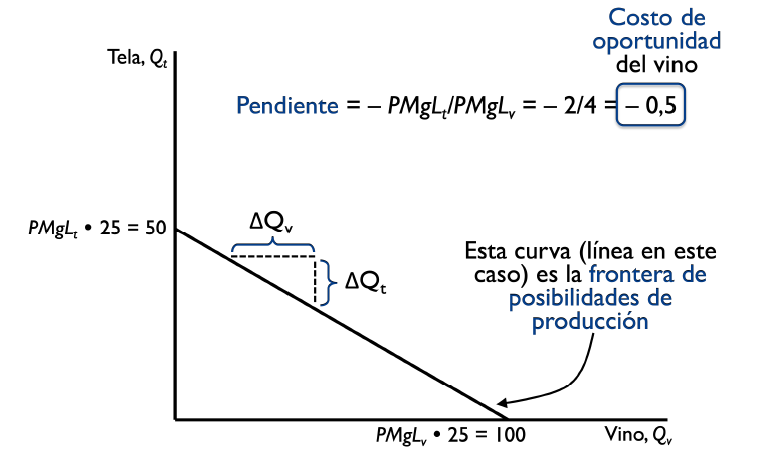
\includegraphics[scale=0.6]{Figures/Tema_03_1_portugal.png}
\end{frame}

\begin{frame}
\frametitle{ Eligiendo en Portugal}
\centering
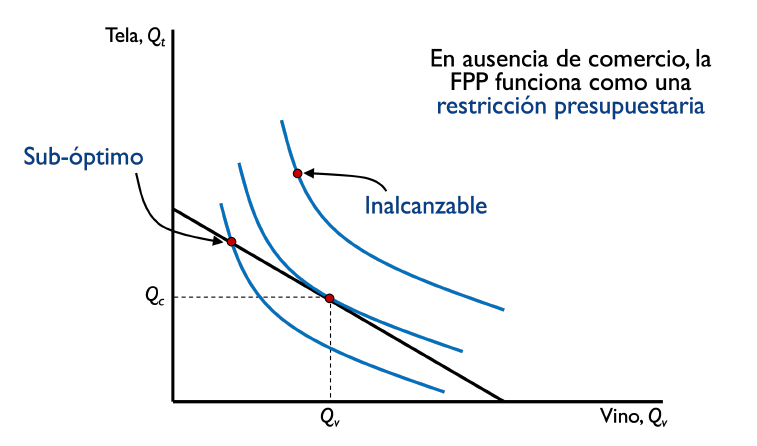
\includegraphics[scale=0.6]{Figures/Tema_03_2_portugal2.png}
\end{frame}

\begin{frame}
\frametitle{ Inglaterra}
\centering
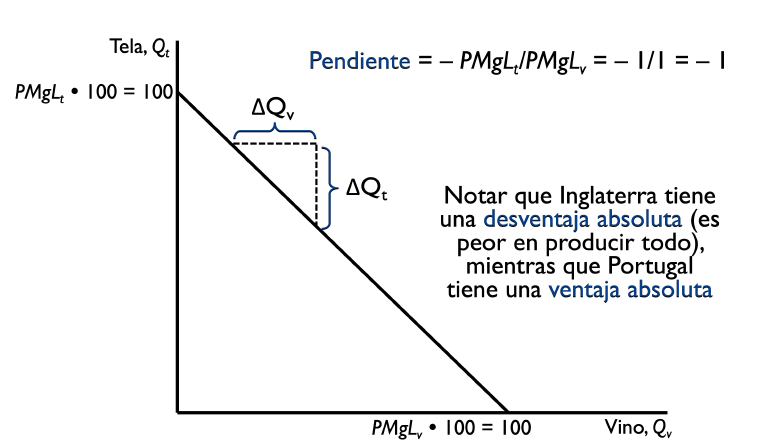
\includegraphics[scale=0.6]{Figures/Tema_03_3_inglaterra.png}
\end{frame}

\begin{frame}
\frametitle{ Eligiendo en Inglaterra}
\centering
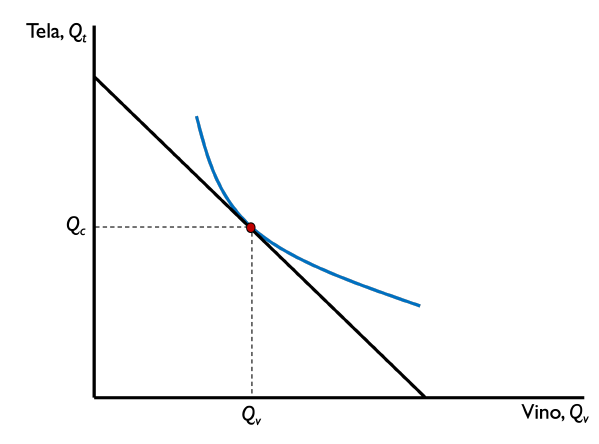
\includegraphics[scale=0.6]{Figures/Tema_03_4_inglaterra2.png}
\end{frame}

\begin{frame}
\frametitle{ Ventaja comparativa}
\begin{itemize}
    \item El costo de oportunidad varía entre los distintos países
    \begin{itemize}
        \item En Inglaterra le toma 1 trabajador producir 1 metro de tela o una botella de vino...
        \item ... pero en Portugal un trabajador produce 2 metros de tela o 4 botellas de vino
    \end{itemize}
    \item Inglaterra tiene una ventaja comparativa en producir tela
    \begin{itemize}
        \item El costo de oportunidad de la tela (1 botella de vino) es menor que en Portugal (2 botellas de vino)
        \item El precio relativo del vino en Inglaterra es mayor que en Portugal
    \end{itemize}
\end{itemize}
\end{frame}

\begin{frame}
\frametitle{Mercado y comercio}
\begin{itemize}
    \item Cada país va a exportar el bien en el cual tiene una ventaja comparativa
    \item Portugal exportará vino, Inglaterra tela
        \begin{itemize}
        \item Productores en Portugal, donde $Pv/Pt = 0,5$ van a querer producir y exportar vino a Inglaterra, donde $Pv/Pt = 1$
        \item Productores en Inglaterra, donde $Pt/Pv = 1$ van a querer producir y exportar tela a Portugal, donde $Pt/Pv = 2$
        \item Los precios de exportación van a subir, mientras que los precios de importación van a bajar
        \end{itemize}
\end{itemize}
\end{frame}

\begin{frame}
\frametitle{Mercado y comercio}
\begin{itemize}
    \item El costo de oportunidad de la tela (1 botella de vino) es menor que en Portugal (2 botellas de vino)
    \item El precio relativo del vino en Inglaterra es mayor que en Portugal
\end{itemize}
\end{frame}

\begin{frame}
\frametitle{ Portugal cuando comercia}
\centering
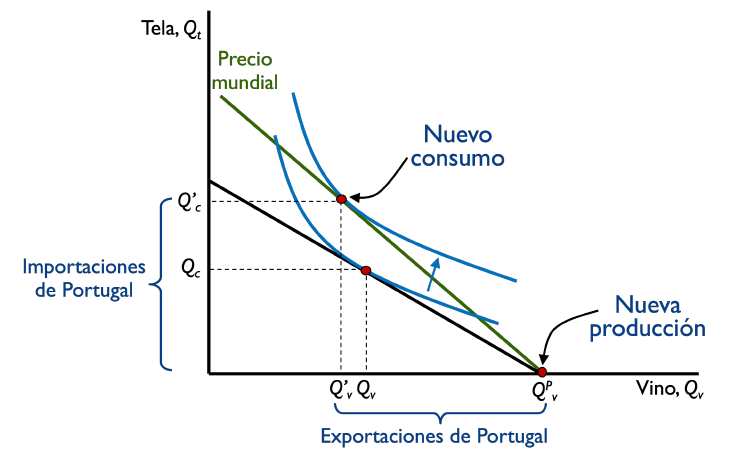
\includegraphics[scale=0.6]{Figures/Tema_03_5_portugal3.png}
\end{frame}

\begin{frame}
\frametitle{Inglaterra cuando comercia}
\centering
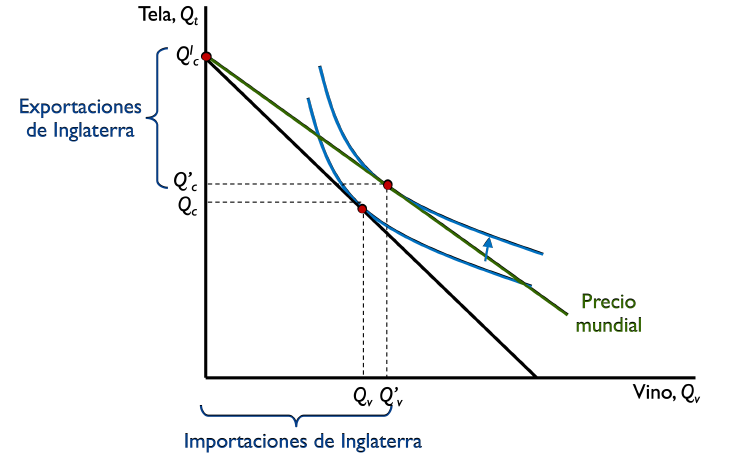
\includegraphics[scale=0.6]{Figures/Tema_03_6_inglaterra3.png}
\end{frame}

\begin{frame}
\frametitle{Conclusiones}
\begin{itemize}
    \item La presencia de mercados logra algo notable: cooperación no intencionada entre extraños
    \item El libre comercio ejemplifica un juego en el que todos los participantes pueden beneficiarse de un escenario en el que todos ganan, todos cooperan para alcanzar el beneficio máximo 
    \item Esto es lo contrario de un juego de suma cero
    \begin{itemize}
    \item La ganancia de un jugador será exactamente igual a la pérdida del otro jugador
    \item Los pagos totales para todos los jugadores en el juego suman cero
    \end{itemize}
\end{itemize}
\end{frame}

\begin{frame}
\frametitle{ Problemas que surgen}
\begin{itemize}
    \item Motivados por interés personal, individuos hacen cosas que pueden afectar a la sociedad
    \item ¿Por qué surgen estos problemas? ¿Qué podemos hacer al respecto?
\end{itemize}
\end{frame}

\begin{frame}
\frametitle{ Dilemas}
\begin{itemize}
    \item Una parte de la economía estudia este tipo de dilemas sociales
    \item Para modelar estos dilemas sociales y distintos tipos de interacciones sociales se suele utilizar lo que se conoce como teoría de juegos
    \end{itemize}
\end{frame}

\begin{frame}
\frametitle{ Teoría de juegos}
\begin{itemize}
\item Estudia de manera formal y abstracta las decisiones óptimas que deben tomar diversos adversarios en conflicto
\item Es el estudio matemático de la toma de decisiones, del conflicto y la estrategia en situaciones sociales
\item Jugadores que toman decisiones que se consideran estratégicas
    \begin{itemize}
        \item los jugadores son entes racionales (no necesariamente humanos)
        \item los entes que participan en el juego actúan teniendo en cuenta las acciones que tomarían los demás
            \end{itemize}
\end{itemize}
\end{frame}

\begin{frame}
\frametitle{ Juegos}
\begin{itemize}
\item Juegos simultáneos donde se toma una decisión one-shot  
\item Juegos secuenciales donde los jugadores toman sus decisiones de forma consecutiva, empleando el principio de inducción hacia atrás
\end{itemize}
\end{frame}

\begin{frame}
\frametitle{ Elementos presentes en un juego}
\begin{itemize}
\item \textbf{Los jugadores:} quién está interactuando con quién
\item \textbf{Las estrategias viables:} qué acciones están abiertas a los jugadores
\item \textbf{La información:} lo que cada jugador sabe al tomar su decisión
\item \textbf{Los beneficios:} cuáles serán los resultados para cada una de las posibles combinaciones de acciones
\end{itemize}
\end{frame}

\begin{frame}
\frametitle{ Estudiando juegos}
\begin{itemize}
\item El término ``juegos'' refiere básicamente a modelos de interacción estratégica
\begin{itemize}
    \item Es decir, modelos donde las personas involucradas en una interacción social saben que sus acciones afectan a otros y viceversa
    \begin{itemize}
        \item En este contexto, una estrategia es una acción (o un curso de acción) que puede tomar una persona cuando es consciente de esta dependencia mutua de los resultados
    \end{itemize}
\end{itemize}
\item ¿Cómo analizamos interacciones sociales?
\begin{itemize}
    \item Definimos las características de un juego
    \item Obtenemos ‘modos de jugar’
    \begin{itemize}
        \item que cumplen con ciertos criterios y nos ayudan a entender si esa manera de jugar es una buena
    \end{itemize}
\end{itemize}
\end{itemize}
\end{frame}


\begin{frame}
\frametitle{ Estudiando juegos}
\begin{itemize}
\item “The Economy” presenta un problema de división de trabajo
\begin{itemize}
    \item Dos individuos deben decidir qué producir, con el riesgo de terminar produciendo lo mismo
        \begin{itemize}
        - ¿Por qué es esto un problema?
        \end{itemize}
        \item Por alguna razón, no se pueden poner de acuerdo
        \begin{itemize}
        - Toman decisiones en forma independiente
        \end{itemize}
        \item Juegan una sola vez
        \end{itemize}
    \item ¿Arroz o mandioca?
        \begin{itemize}
        \item Asumimos que ninguno puede producir ambos...
        \item ... y que Bala es mejor produciendo arroz, mientras que Anil es mejor produciendo mandioca
    \end{itemize}
\end{itemize}
\end{frame}

\begin{frame}
\frametitle{ Escenarios}
\centering
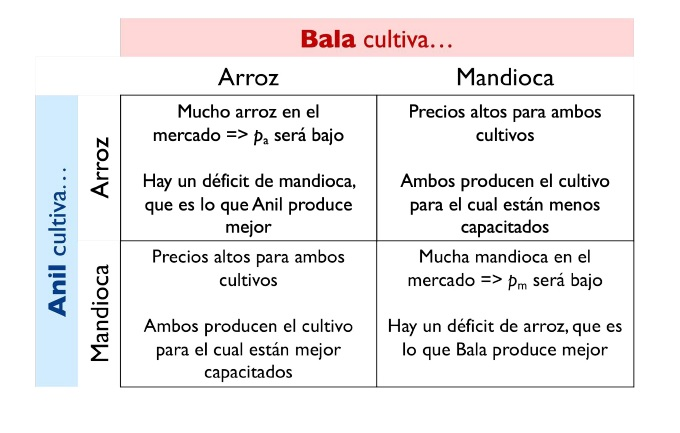
\includegraphics[scale=0.65]{Figures/Tema_03_7_bala.jpg}
\end{frame}

\begin{frame}
\frametitle{26. El juego de Anil y Bala}
\begin{itemize}
    \item Jugadores
        \begin{itemize}
        \item Anil y Bala, dos agricultores que deciden en qué cultivo especializarse
        \end{itemize}
    \item Estrategias viables
        \begin{itemize}
        \item Arroz o mandioca
        \end{itemize}
    \item Información
        \begin{itemize}
        \item Ningún agricultor sabe lo que el otro elige
        \end{itemize}
    \item Pagos
        \begin{itemize}
        \item Dependerá de los precios de mercado y de la calidad de la tierra
        \end{itemize}
\end{itemize}
\end{frame}

\begin{frame}
\frametitle{ Construyendo la matriz de pagos}
\centering
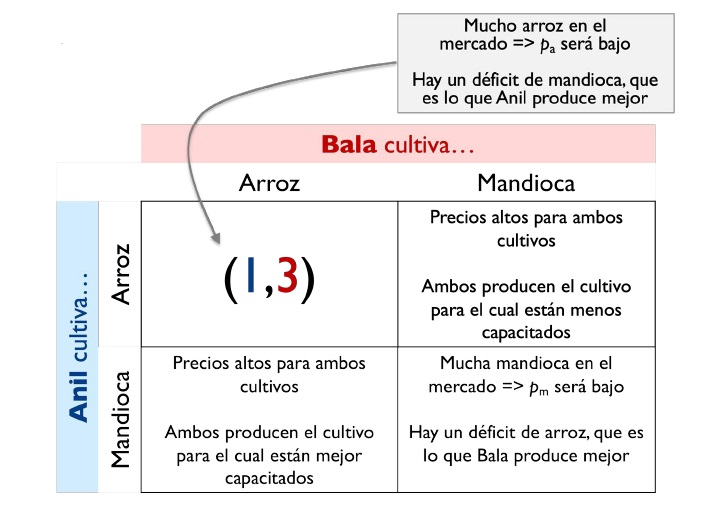
\includegraphics[scale=0.6]{Figures/Tema_03_8_bala.jpg}
\end{frame}

\begin{frame}
\frametitle{28. Construyendo la matriz de pagos}
\centering
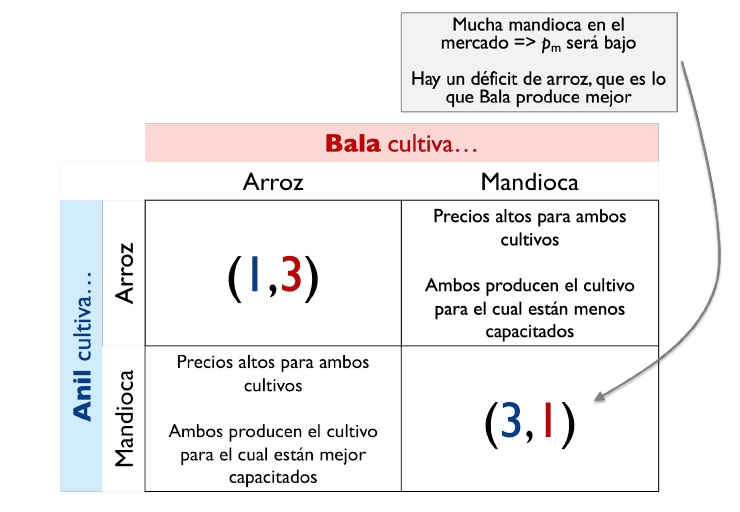
\includegraphics[scale=0.6]{Figures/Tema_03_9_bala.jpg}
\end{frame}

\begin{frame}
\frametitle{ Construyendo la matriz de pagos}
\centering
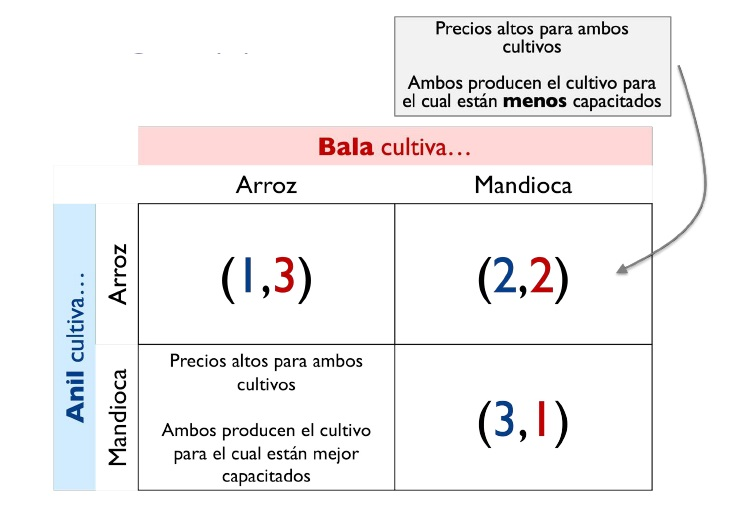
\includegraphics[scale=0.6]{Figures/Tema_03_10_bala.jpg}
\end{frame}

\begin{frame}
\frametitle{Construyendo la matriz de pagos}
\centering
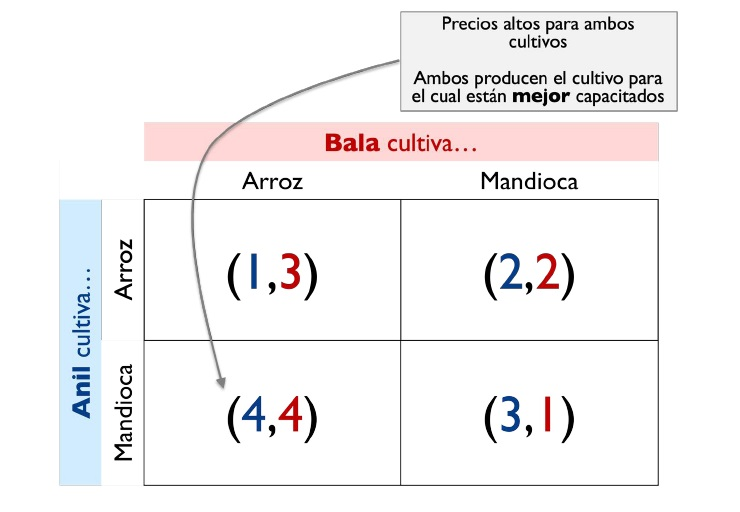
\includegraphics[scale=0.6]{Figures/Tema_03_11_bala.jpg}
\end{frame}

\begin{frame}
\frametitle{Matriz de pagos}
\centering
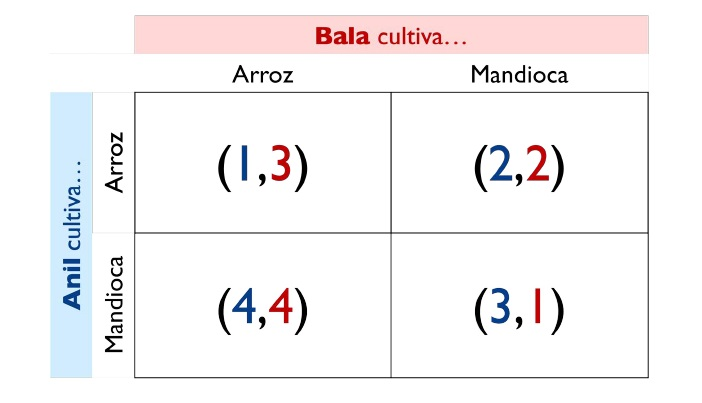
\includegraphics[scale=0.6]{Figures/Tema_03_12_bala.jpg}
\end{frame}

\begin{frame}
\frametitle{¿Cómo pensamos el problema?}
\begin{itemize}
    \item ¿Cuál es la mejor respuesta de cada individuo?
        \begin{itemize}
        \item Aquella estrategia que brinda los mayores pagos, dada la estrategia seleccionada por la otra persona
        \end{itemize}
    \item A veces, existe una estrategia dominante
        \begin{itemize}
        \item Esta es una mejor respuesta a todas las posibles estrategias de otro jugador
        \end{itemize}
    \item Si se encuentra un resultado donde cada individuo juega su estrategia dominante, entonces nos encontramos con un equilibrio en estrategia dominante
\end{itemize}
\end{frame}

\begin{frame}
\frametitle{ ¿Cómo piensa Anil?}
\centering
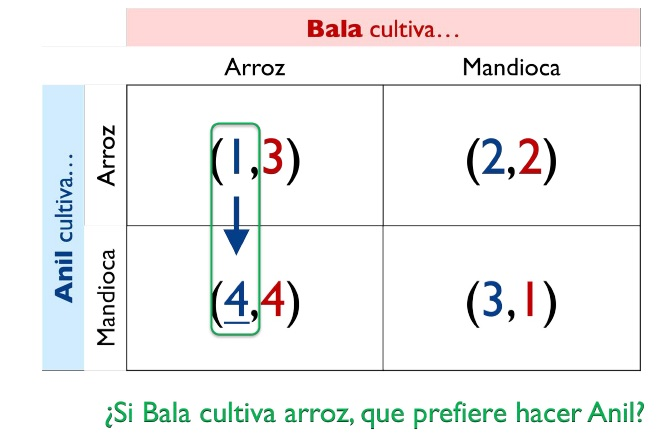
\includegraphics[scale=0.6]{Figures/Tema_03_13_bala.jpg}
\end{frame}

\begin{frame}
\frametitle{ ¿Cómo piensa Anil?}
\centering
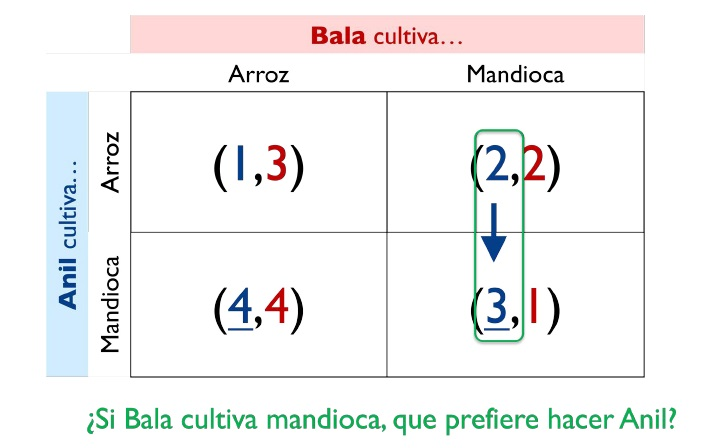
\includegraphics[scale=0.6]{Figures/Tema_03_14_bala.jpg}
\end{frame}

\begin{frame}
\frametitle{ ¿Qué hace Anil?}
\centering
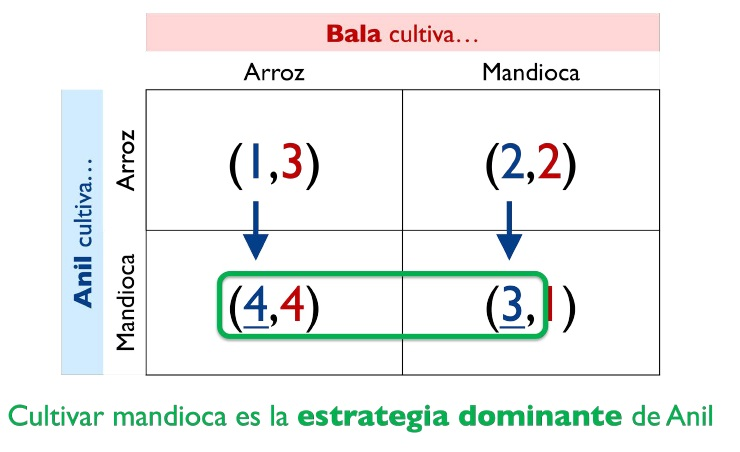
\includegraphics[scale=0.6]{Figures/Tema_03_15_bala.jpg}
\end{frame}

\begin{frame}
\frametitle{ ¿Cómo piensa Bala?}
\centering
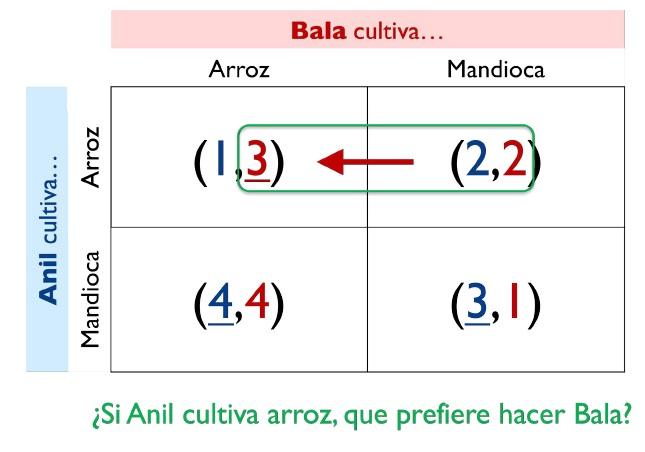
\includegraphics[scale=0.6]{Figures/Tema_03_16_bala.jpg}
\end{frame}

\begin{frame}
\frametitle{ ¿Cómo piensa Bala?}
\centering
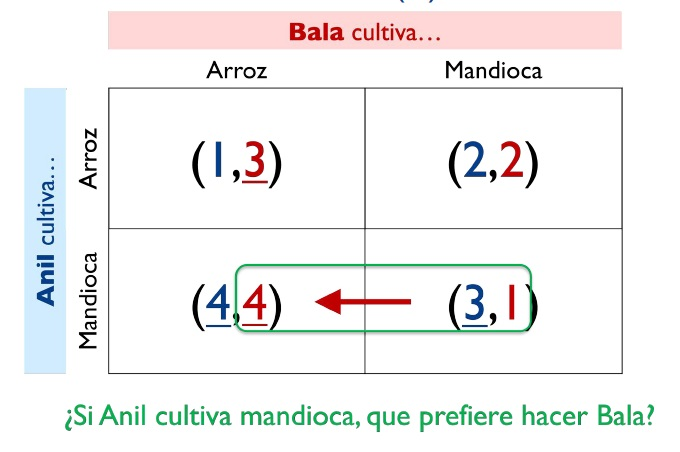
\includegraphics[scale=0.6]{Figures/Tema_03_17_bala.jpg}
\end{frame}

\begin{frame}
\frametitle{ ¿Qué hace Bala?}
\centering
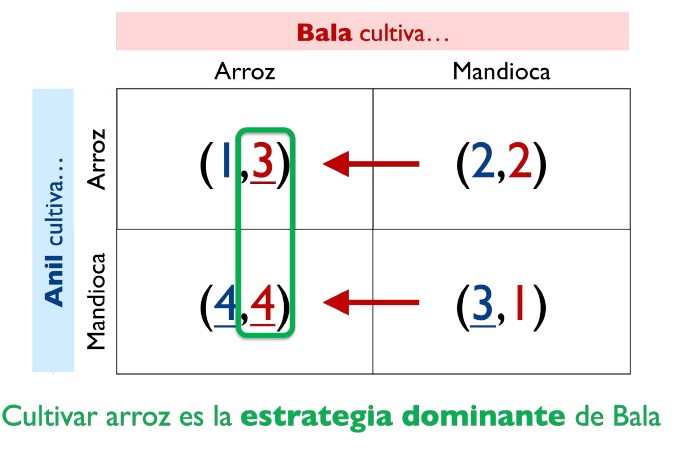
\includegraphics[scale=0.6]{Figures/Tema_03_18_bala.jpg}
\end{frame}

\begin{frame}
\frametitle{Equilibrio}
\centering
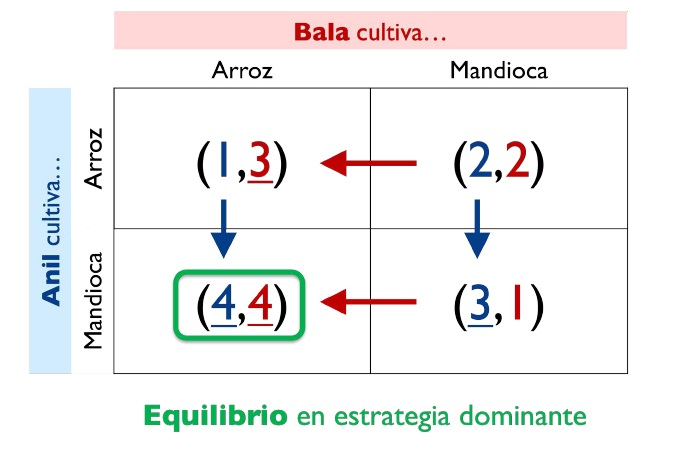
\includegraphics[scale=0.6]{Figures/Tema_03_19_bala.jpg}
\end{frame}

\begin{frame}
\frametitle{ Otro juego}
\begin{itemize}
    \item Dos empresas productoras de \textit{smartphones}
    \item Comparten por igual el mercado de un país por, digamos, \$8 millones
    \item Enfrentan el problema de invertir en publicidad
        \begin{itemize}
        \item Si ambos invierten en publicidad, mantienen su proporción del mercado inalterada
        \item Si uno de ellos invierte  \$1 millón, se queda con $\frac{3}{4}$ del mercado
        \end{itemize}
    \item ¿Cómo analizamos este caso?    
\end{itemize}
\end{frame}

\begin{frame}
\frametitle{ El juego de Apple y Samsung}
\begin{itemize}
    \item Jugadores
        \begin{itemize}
        \item Apple y Samsung, dos compañías que quieren maximizar su participación en el mercado
        \end{itemize}
    \item Estrategias viables
        \begin{itemize}
        \item Publicitar o no publicitar
        \end{itemize}
    \item Información
        \begin{itemize}
        \item Ambos tienen la misma información, y ninguno puede ver la decisión del otro antes de jugar
        \end{itemize}
    \item Pagos
        \begin{itemize}
        \item Dependerá del costo de publicidad y el mercado
        \end{itemize}
\end{itemize}
\end{frame}

\begin{frame}
\frametitle{ Matriz de pagos}
\centering
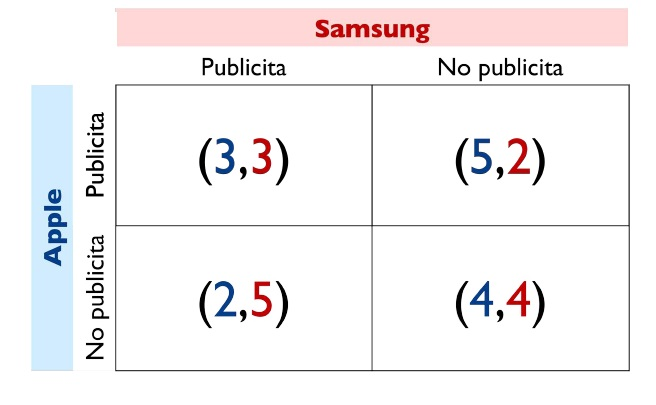
\includegraphics[scale=0.6]{Figures/Tema_03_20_bala.jpg}
\end{frame}

\begin{frame}
\frametitle{ Equilibrio}
\centering
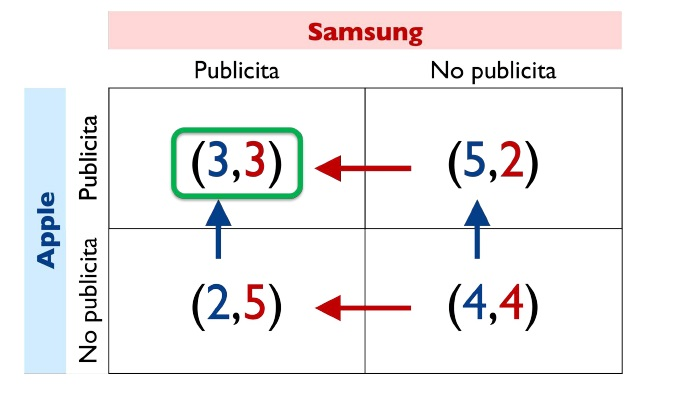
\includegraphics[scale=0.6]{Figures/Tema_03_21_bala.jpg}
\end{frame}

\begin{frame}
\frametitle{Dilema del prisionero}
\begin{itemize}
    \item Este ejemplo de las empresas de \textit{smartphones} es un dilema del prisionero disfrazado
        \begin{itemize}
        \item Típicamente, un juego con un equilibrio en estrategia dominante donde el resultado son pagos individuales y totales inferiores a otras estrategias posibles
        \end{itemize}
        \end{itemize}
        \textbf{El resultado socialmente óptimo no es alcanzado} \vspace{2mm}
        \begin{itemize}
        \item Este tipo de dilema es útil para representar una serie de problemáticas sociales
        \begin{itemize}
        \item Desde temas ambientales hasta conflictos en la provisión de algunos tipos de bienes
        \end{itemize}
\end{itemize}
\end{frame}

\begin{frame}
\frametitle{Problemas y soluciones}
\begin{itemize}
    \item ¿Por qué se llega a este tipo de resultado y en qué forma se puede amenorar o solucionar?
    \item Algunas razones (y soluciones)
        \begin{itemize}
        \item Los jugadores sólo se preocupan por sus propios beneficios \\
        - Podemos introducir preferencias sociales
        \item Nadie puede hacer que los jugadores paguen por las consecuencias de sus acciones sobre los demás \\
        - Juegos repetidos, normas sociales y castigo de pares
        \item Los jugadores no pueden coordinar sus acciones con antelación \\
        - Cambiar las reglas del juego (instituciones y políticas)
        \end{itemize}
\end{itemize}
\end{frame}

\begin{frame}
\frametitle{Asfaltando la calle}
\begin{itemize}
    \item Dos familias viven en una calle de tierra (Álvarez y Benítez)
    \item Ambas se beneficiarían si se asfaltara la calle
        \begin{itemize}
        \item Por ejemplo, tendrían que gastar menos en arreglo y limpieza de sus autos por \$15.000
        \end{itemize}
    \item Enfrentan el problema de invertir en el asfalto
        \begin{itemize}
        \item El costo de asfaltar la calle es de \$20.000
        \item Puede pagarlo una u otra familia, o las dos juntas
        \end{itemize}
\item ¿Cómo analizamos este caso?
\end{itemize}
\end{frame}

\begin{frame}
\frametitle{ El juego del asfalto}
\begin{itemize}
    \item Jugadores
        \begin{itemize}
        \item Familias Álvarez y Benítez
        \end{itemize}
    \item Estrategias viables
        \begin{itemize}
        \item Pagar o no pagar por el asfalto
        \end{itemize}
    \item Información
        \begin{itemize}
        \item Ambos tienen la misma información, y ninguno puede ver la decisión del otro antes de jugar
        \end{itemize}
    \item Pagos
        \begin{itemize}
        \item Dependerá del ahorro en arreglos del auto y la contribución al costo del asfalto
        \end{itemize}
\end{itemize}
\end{frame}

\begin{frame}
\frametitle{ Pagando por el asfalto}
\centering
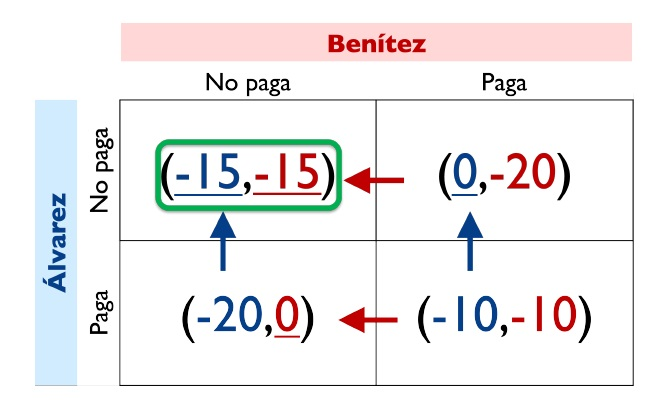
\includegraphics[scale=0.6]{Figures/Tema_03_27_abel.jpg}
\end{frame}

\begin{frame}
\frametitle{El problema del bien público}
\begin{itemize}
    \item Existe un tipo de bien, usualmente llamado bien público, con dos características distintivas:
    \begin{itemize}
        \item Es no rival \\
        - Su uso por una persona no perjudica o impide el uso simultáneo por parte de otros individuos
        \item Es no excluyente \\
        - No se puede impedir ser utilizado
    \end{itemize}
    \item El dilema del prisionero ilustra un problema de los bienes públicos: pueden no producirse
    \begin{itemize}
        \item Dadas sus característica, existe la posibilidad de hacer free-riding \\
        - ¡No contribuir es la estrategia dominante!
    \end{itemize}
\end{itemize}
\end{frame}

\begin{frame}
\frametitle{ Pagando por los costos que uno genera}
\begin{itemize}
    \item Tanto en el caso del asfalto, como en el de los pesticidas elaborado en “The Economy”: \\
\end{itemize}
\vspace{5mm}
\textbf{Es difícil hacer pagar a los jugadores por la
consecuencias de sus acciones sobre los demás}
\end{frame}

\begin{frame}
\frametitle{ Mitigando el problema}
\begin{itemize}
    \item Mecanismos ayudan a reducir el problema
    \begin{itemize}
        \item Juegos repetidos \\
        - Repetición contribuye a la cooperación: las consecuencias en el futuro hacen la estrategia egoísta sub-óptima
        \item Normas sociales \\
        - Reglas que indican como actuar en contextos particulares \\
        - Individuos a veces incurren en considerables costos para castigar a pares que violan normas sociales o llevan a cabo acciones que consideran injustas (¿gusto por equidad?)
    \end{itemize}
\end{itemize}
\end{frame}

\begin{frame}
\frametitle{ Aprendiendo sobre preferencias}
\begin{itemize}
    \item Los economistas utilizan a veces experimentos para aprender sobre las preferencias
    \begin{itemize}
        \item En el laboratorio: \\
        - Se puede controlar las decisiones de los participantes y sus resultados \\
        - Se puede crear un grupo de control / tratamiento para la comparación \\
        - Los resultados pueden ser replicados \\
        - Se pueden controlar otras variables
        \item En el campo \\
        - Algunos experimentos de laboratorio no pueden predecir la toma de decisiones en el mundo real \\
        - El campo provee un contexto más realista en el que las personas toman decisiones
    \end{itemize}
\end{itemize}
\end{frame}

\begin{frame}
\frametitle{ El dilema de la guardería}
\begin{itemize}
    \item Un experimento `real' (`field experiment')
       \begin{itemize}
       \item Se introdujo una multa a la llegada tarde de los padres... con un resultado no esperado \\
        - ¡Más padres empezaron a llegar tarde!
        \end{itemize}
    \item ¿Por qué?
        \begin{itemize}
        \item Antes del experimento, llegar tarde era `incorrecto' 
        \item El tiempo de los maestros pasó a tener un valor definido \\
        - El precio del retardo, que los padres podían estar dispuestos a pagar o no \\ 
        \item En este caso, se dice que los incentivos hicieron un crowding out de las preferencias sociales
    \end{itemize}
\end{itemize}
\end{frame}

\begin{frame}
\frametitle{ En el campo ... con padres y niños}
\centering
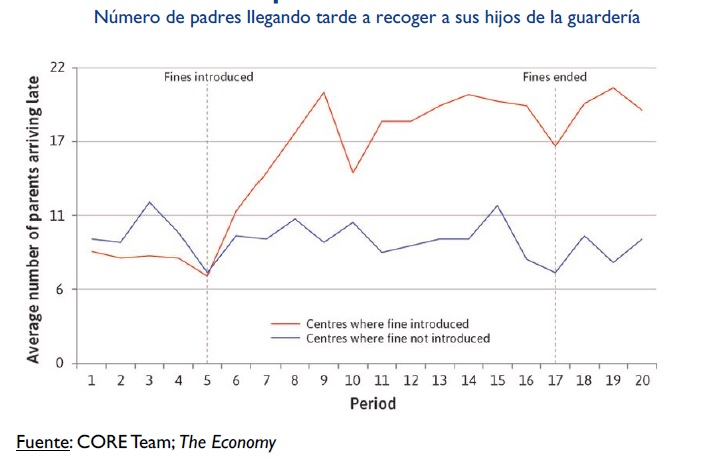
\includegraphics[scale=0.6]{Figures/Tema_03_28_guarderia.jpg}
\end{frame}

\begin{frame}
\frametitle{55. Negociando}
\begin{itemize}
    \item La cooperación es posible aun cuando agentes 
    actúan en forma independiente
    \begin{itemize}
        \item En muchos de los ejemplos que discutimos no fue necesario que los individuos se pusieran de acuerdo \\
        - A veces las condiciones del juego ayudaban (con Anil y Bala), o si se repetía el juego, o si permitía sancionar a los que no colaboraban
    \end{itemize}
    \item Pero la negociación es otra herramienta para conseguir un acuerdo mutuamente beneficioso
    \begin{itemize}
        \item Más fácil decirlo que hacerlo \\
        - ¿Cómo repartir los costos y beneficios de la interacción?
    \end{itemize}
\end{itemize}
\end{frame}

\begin{frame}
\frametitle{Motivando preferencias sociales}
\begin{itemize}
        \item Altruismo
        \begin{itemize}
            \item Una persona puede ser altruista y preocuparse de la felicidad (o sobre algún otro aspecto del bienestar) de los demás
        \end{itemize}
        \item Equidad
        \begin{itemize}
            \item La importancia de distribuir recursos en forma justa \\
            - Motivación por lo que los economistas llaman `aversión por la desigualdad'
        \end{itemize}
        \item Reciprocidad
        \begin{itemize}
            \item Existencia de preferencias recíprocas \\
            - Si en el pasado han sido generosos con nosotros, merecemos tratar en forma generosa
        \end{itemize}
\end{itemize}
\end{frame}

\begin{frame}
\frametitle{ Juego del ultimátum}
\begin{itemize}
        \item Una herramienta muy utilizada para estudiar preferencias sociales es el juego del ultimátum
        \begin{itemize}
            \item ü Dos jugadores, seleccionados aleatoriamente \\ 
            - Proponente \\
            - Receptor
            \item El proponente recibe algo de valor (típicamente dinero) y debe ofrecerle al receptor una parte \\
            - Que puede ser cualquier cosa entre todo y nada \\
            - El receptor sabe cuán grande es el total
            \item Una vez que el receptor escucha la oferta, decide si la acepta o no \\
            - Si la oferta es rechazada, nadie recibe nada \\
            - Si es aceptada, se reparte como sugirió el proponente
        \end{itemize}
\end{itemize}
\end{frame}

\begin{frame}
\frametitle{ Juego secuencial}
\centering
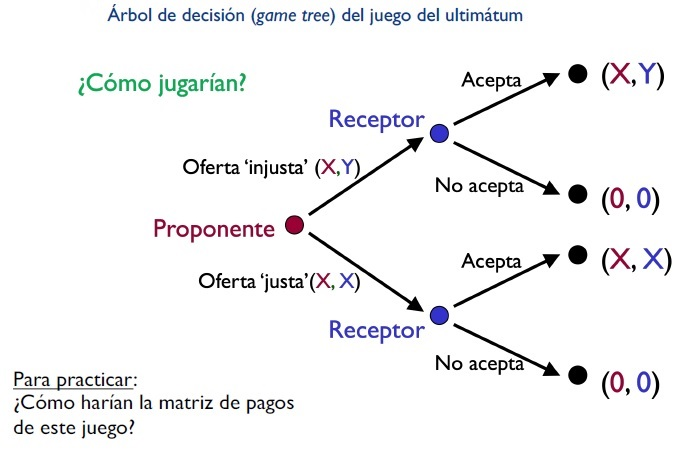
\includegraphics[scale=0.6]{Figures/Tema_03_29_arbol.jpg}
\end{frame}

\begin{frame}
\frametitle{ Agricultores versus estudiantes}
\centering
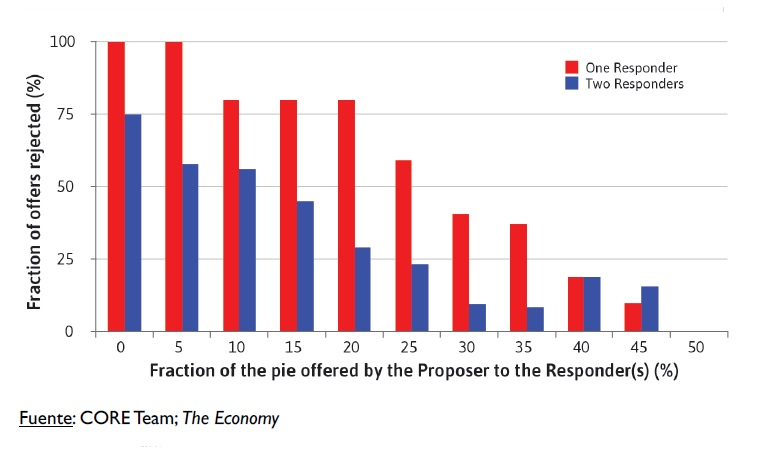
\includegraphics[scale=0.6]{Figures/Tema_03_32_ultimatum.jpg}
\end{frame}

\begin{frame}
\frametitle{ ¿Cuál es el beneficio esperado?}
\centering
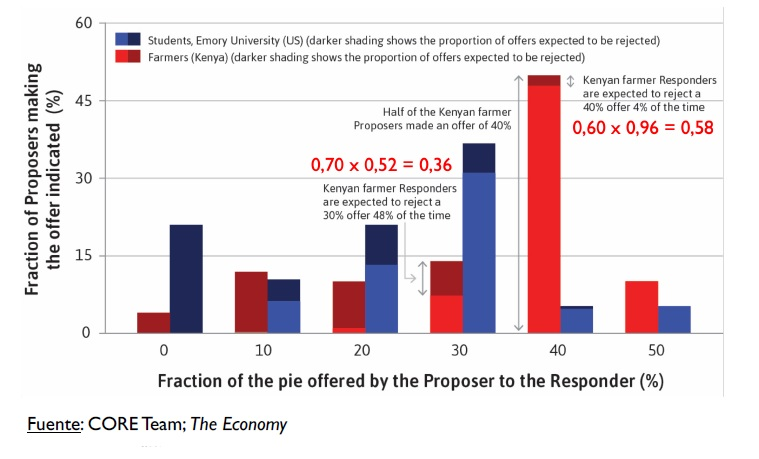
\includegraphics[scale=0.6]{Figures/Tema_03_31_ultimatum.jpg}
\end{frame}

\begin{frame}
\frametitle{ ¿Y si hay competencia?}
\centering
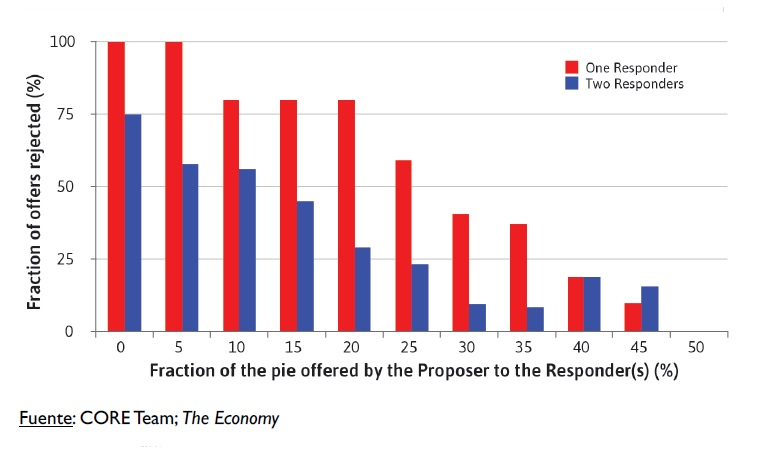
\includegraphics[scale=0.6]{Figures/Tema_03_32_ultimatum.jpg}
\end{frame}

\begin{frame}
\frametitle{Equilibrio de Nash}
\begin{itemize}
        \item Hasta ahora, siempre encontramos un equilibrio en estrategias dominantes
        \begin{itemize}
            \item Existía una estrategia dominante para los jugadores
        \end{itemize}
        \item Existe otro concepto de equilibrio que suele ser útil, el equilibrio de Nash
        \end{itemize}
\textbf{Resultado de un juego donde ninguno de los jugadores desea jugar de manera distinta, dadas las acciones de cada uno de los demás jugadores} \vspace{2mm}
\begin{itemize}
        \begin{itemize}
            \item Cada jugador ha adoptado su mejor estrategia \\
            - Por lo cual, ningún jugador gana cambiando su estrategia si nadie más cambia la suya
        \end{itemize}
        \end{itemize}
\end{frame}

\begin{frame}
\frametitle{ La batalla de los sexos}
\begin{itemize}
        \item Una pareja arregló para ir al cine
        \begin{itemize}
            \item Alberto y Beatriz
        \end{itemize}
        \item No recuerdan qué película iban a ver
        \begin{itemize}
            \item Alberto quería ir a ver una comedia romántica
            \item Beatriz una de acción
        \end{itemize}
        \item Ambos prefieren ir al mismo lugar que desencontrarse
        \item No tienen forma de comunicarse
        \item ¿Cómo analizamos este caso?
\end{itemize}
\end{frame}

\begin{frame}
\frametitle{¿Y si hay competencia?}
\centering
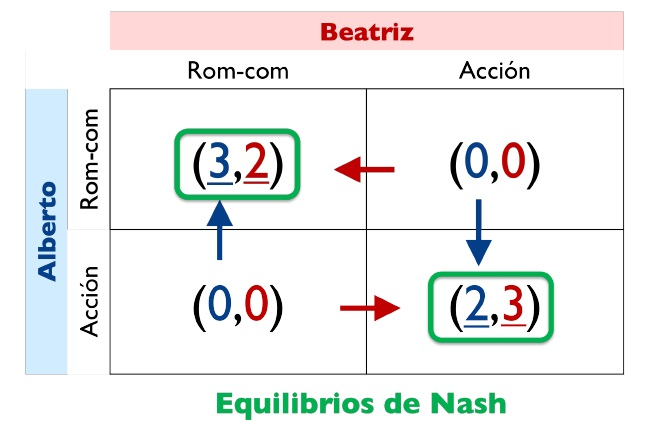
\includegraphics[scale=0.6]{Figures/Tema_03_33_batallasexo.jpg}
\end{frame}

\begin{frame}
\frametitle{Juegos de coordinación}
\begin{itemize}
        \item La batalla de los sexos es un típico juego de coordinación
        \begin{itemize}
            \item Ilustra situaciones que encontramos por doquier en la sociedad \\
            - ¿Qué plataforma de social media usar? ¿De qué lado del camino conducir?
        \end{itemize}
        \item En este caso, el pago era idéntico en ambos equilibrios, pero puede que los jugadores queden atrapados en un mal equilibrio
        \begin{itemize}
            \item ¿Cómo se decide, por ejemplo, pasar de una tecnología a otra cuando la nueva implica un costo para el capitalista y para el trabajador?
        \end{itemize}
\end{itemize}
\end{frame}

\begin{frame}
\frametitle{Juegos de coordinación}
\begin{itemize}
        \item La batalla de los sexos es un típico juego de coordinación
        \begin{itemize}
            \item Ilustra situaciones que encontramos por doquier en la sociedad \\
            - ¿Qué plataforma de social media usar? ¿De qué lado del camino conducir?
        \end{itemize}
        \item En este caso, el pago era idéntico en ambos equilibrios, pero puede que los jugadores queden atrapados en un mal equilibrio
        \begin{itemize}
            \item ¿Cómo se decide, por ejemplo, pasar de una tecnología a otra cuando la nueva implica un costo para el capitalista y para el trabajador?
        \end{itemize}
\end{itemize}
\end{frame}

\begin{frame}
\frametitle{Inversión en nueva tecnología}
\begin{itemize}
        \item Dos tipos de agente en la economía
        \begin{itemize}
            \item Capitalistas y trabajadores
        \end{itemize}
        \item Se está considerando introducir una nueva tecnología
        \begin{itemize}
            \item Ésta aumenta la productividad del trabajador y permite al capitalista producir a un menor costo
        \end{itemize}
        \item La tecnología no es gratuita para ninguno
        \begin{itemize}
            \item El costo del capital para el capitalista
            \item La inversión en capital humano para el trabajador
        \end{itemize}
        \item ¿Cómo analizamos este caso?
\end{itemize}
\end{frame}

\begin{frame}
\frametitle{Cambio tecnológico}
\centering
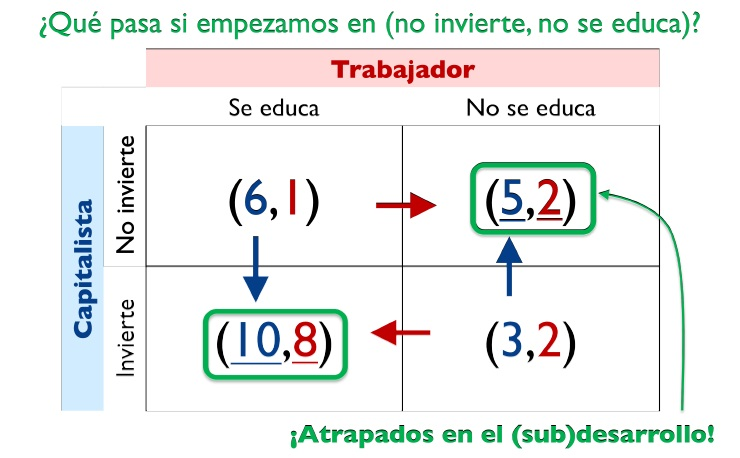
\includegraphics[scale=0.6]{Figures/Tema_03_34_catecno.jpg}
\end{frame}

\begin{frame}
\frametitle{Asignaciones}
\begin{itemize}
    \item Una asignación es el resultado de una interacción económica, la cual está determinada por distintos factores:
    \begin{itemize}
        \item La tecnología y la biología determinan lo posible...
        \item ... las instituciones restringen el accionar de los agentes ...
        \item ... y las preferencias los motivan a interactuar
    \end{itemize}
    \item Generalmente, estamos interesados en al menos dos aspectos de estos factores:
    \begin{itemize}
        \item Querríamos describirlas \\
        ¿Quién hace qué? ¿Quién obtiene qué?
        \item Querríamos evaluarlas \\ 
        ¿Es mejor o peor que otras potenciales asignaciones?
    \end{itemize}
\end{itemize} 
\end{frame}

\begin{frame}
\frametitle{ Factores que determinan una asignación}
\definecolor{Azul}{rgb}{0.1,0.1,0.6}
\begin{itemize}
    \item Instituciones
    \item \textcolor{Azul}{Tecnología}
    \item \textcolor{Azul}{Biología}
    \item \textcolor{Azul}{Preferencias}
\end{itemize} 
\end{frame}

\begin{frame}
\frametitle{Un nuevo modelo}
\begin{itemize}
    \item ¿Qué se puede producir? \vspace{2mm}
        \begin{itemize}
        \item La frontera factible nos indica lo que es tecnológicamente posible \vspace{2mm}
        \item Pero ahora vamos a considerar lo que es biológicamente posible
        \begin{itemize} \vspace{2mm}
            \item ¿Qué significa esto? \\
            - Hay un mínimo de recursos que el individuo necesita para sobrevivir, aún si no produce nada...
            - ... y cuantas mas energías utiliza produciendo, más recursos va a necesitar
        \end{itemize}
    \end{itemize}
\end{itemize}
\end{frame}

\begin{frame}
\frametitle{ Cuando importa la biología}
\centering
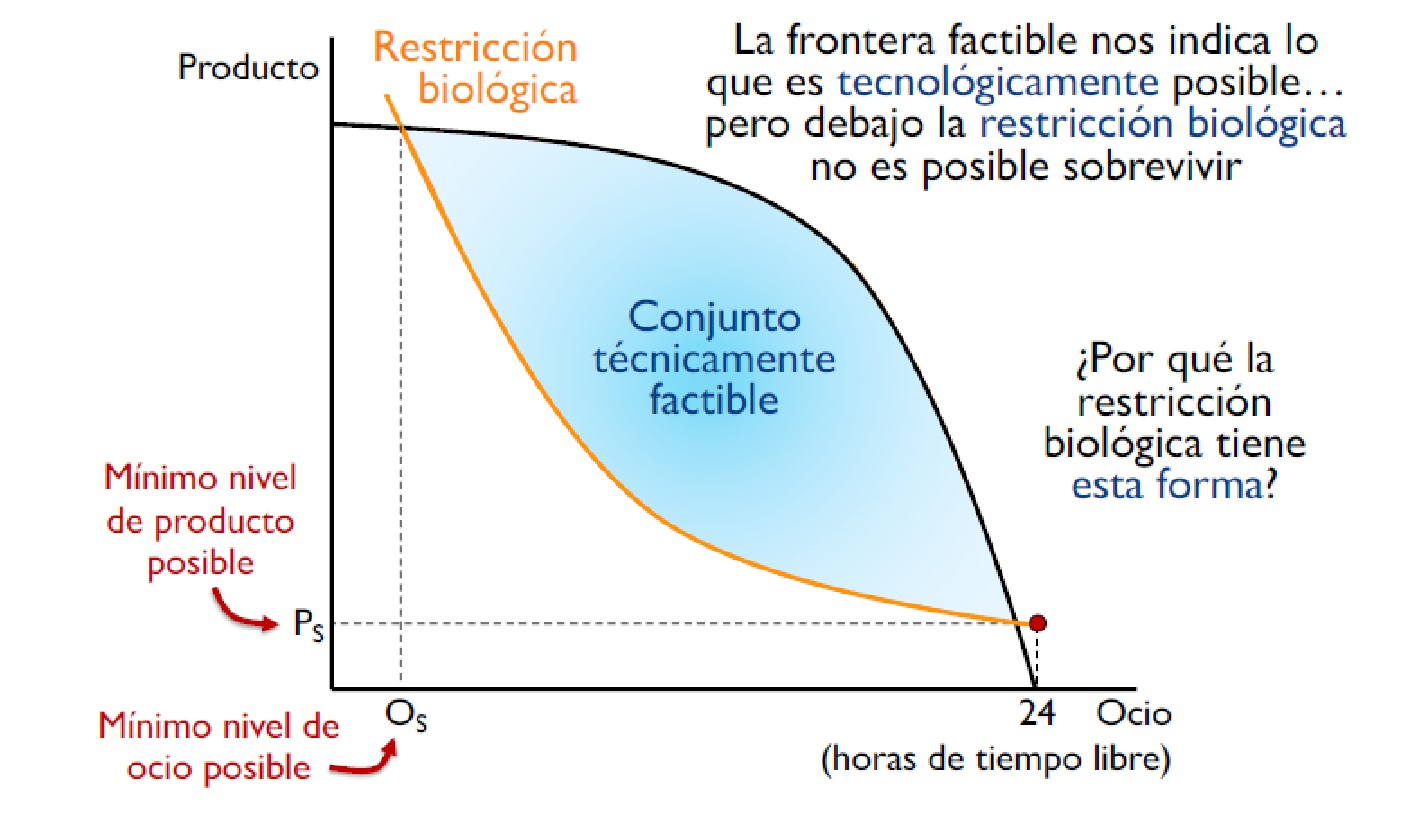
\includegraphics[scale=0.3]{Figures/Tema_04.4_tecnoybiologia.jpg}
\end{frame}

\begin{frame}
\frametitle{¿Y cuando hay otra alternativa?}
\centering
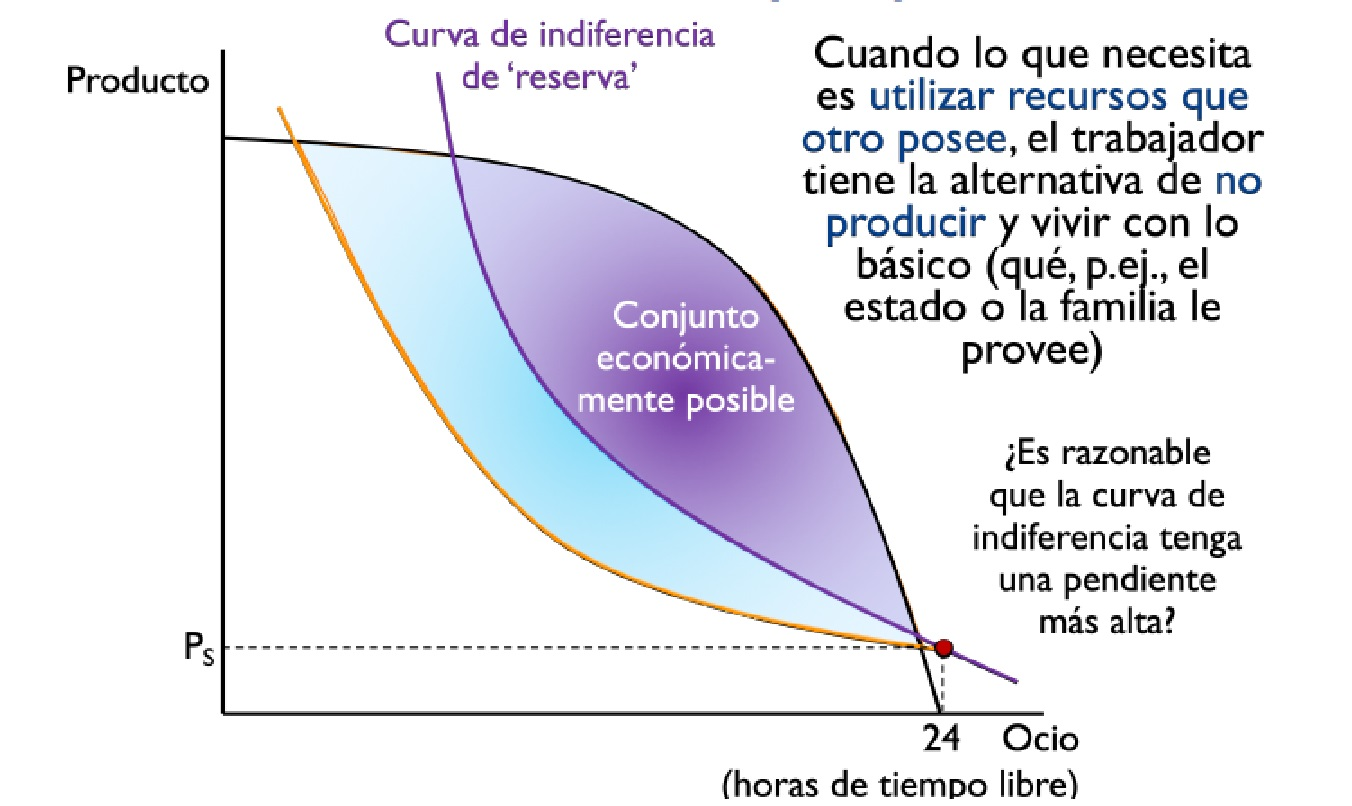
\includegraphics[scale=0.3]{Figures/Tema_04.10_modcap4_5.jpg}
\end{frame}


\begin{frame}
\frametitle{ El modelo}
\begin{itemize}
        \item ¿Cómo lucen las preferencias? \vspace{2mm}
        \begin{itemize}
            \item Vamos a hacer un supuesto sobre la forma de las curvas de indiferencia para simplificar toda la interpretación \\ \vspace{2mm}
            - Tener más o menos producto no va a afectar la valuación del ocio, es decir, valoramos el ocio siempre igual, independientemente del nivel de producto (es decir, TMS constante para un nivel de ocio)
        \end{itemize}
\end{itemize}
\end{frame}

\begin{frame}
\frametitle{Preferencias cuasi-lineales}
\centering
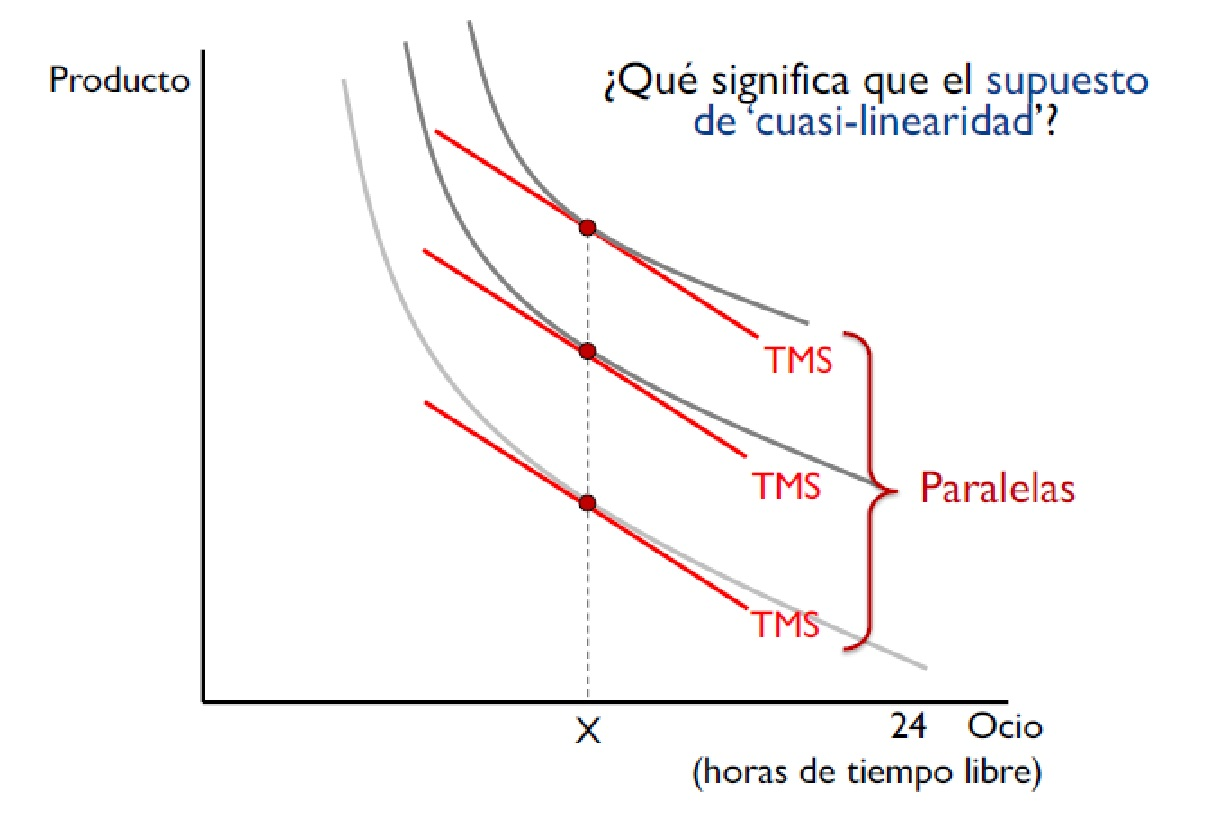
\includegraphics[scale=0.3]{Figures/Tema_04.5_prefcuasilin.jpg}
\end{frame}

\begin{frame}
\frametitle{ El objetivo es comparar las distintas instituciones}
\begin{itemize}
        \item Comparamos escenarios donde:
            \begin{itemize}
            \item Base 1: un agente con acceso a insumos decide solo cuanto producir
            \item Base 2: un agente que decide cuánto se trabaja
            \item Situaciones históricas
            \begin{itemize}
            \item Esclavitud
            \item Servidumbre con renta fija
            \item Servidumbre con renta variable
            \item Tazón de hierro
            \item Sindicatos
            \end{itemize}
        \end{itemize}
    \item ¿En qué forma queremos compararlas? Por ahora, en términos de eficiencia de Pareto
\end{itemize}
\end{frame}

\begin{frame}
\frametitle{ Base 1: Elección individual}
\centering
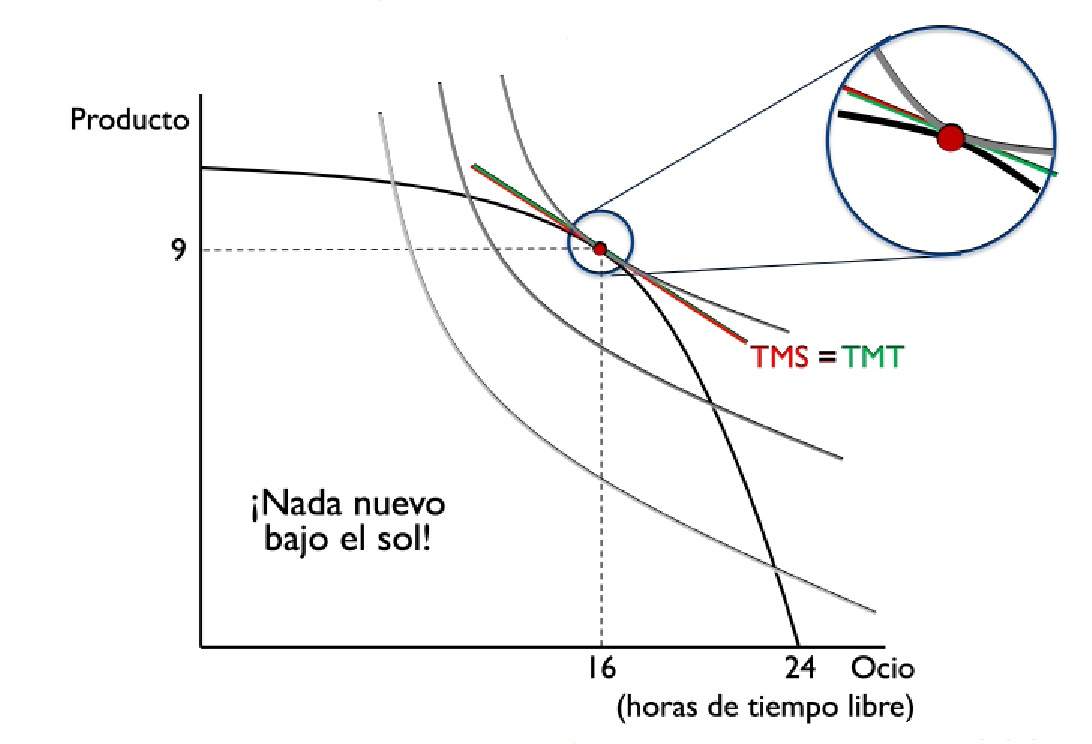
\includegraphics[scale=0.35]{Figures/Tema_04.6_modcap4.jpg}
\end{frame}

\begin{frame}
\frametitle{ Base 2: Imposición por fuerza}
\centering
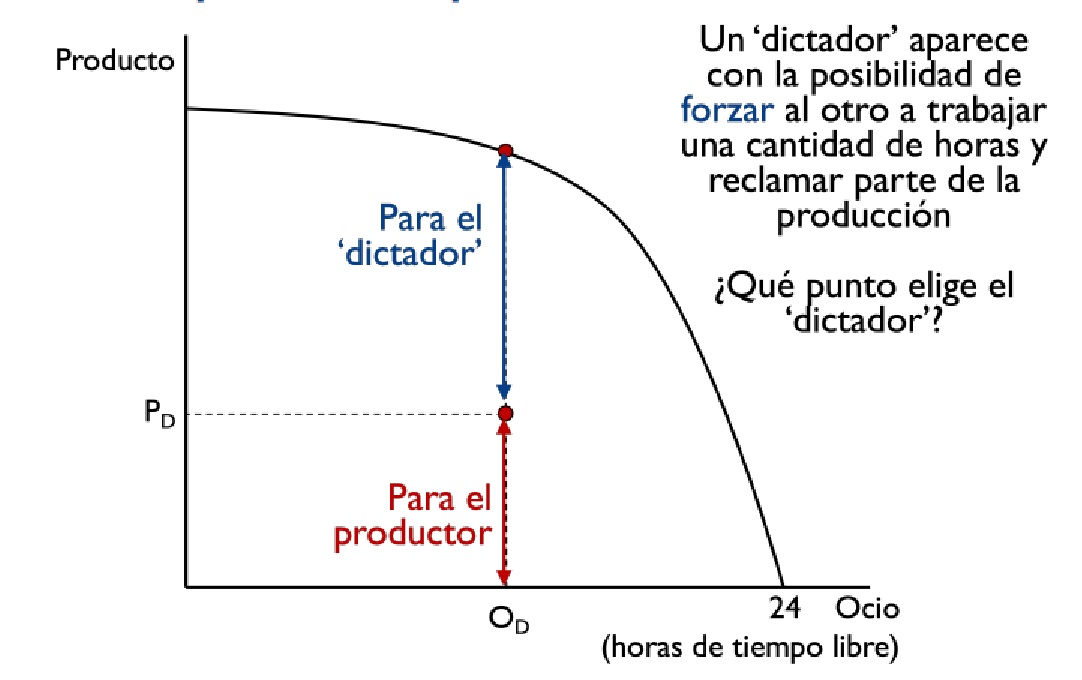
\includegraphics[scale=0.4]{Figures/Tema_04.7_modcap4_2.jpg}\end{frame}

\begin{frame}
\frametitle{ Esclavitud}
\centering
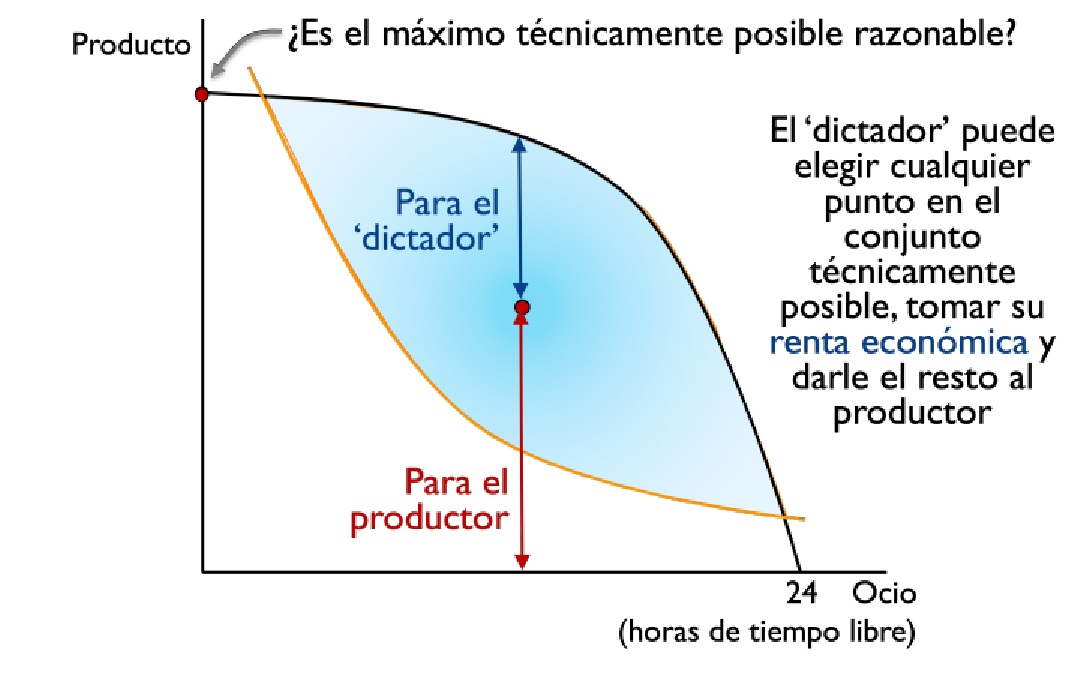
\includegraphics[scale=0.4]{Figures/Tema_04.8_modcap4_3.jpg}
\end{frame}

\begin{frame}
\frametitle{ ¿Cómo se maximiza el excedente?}
\centering
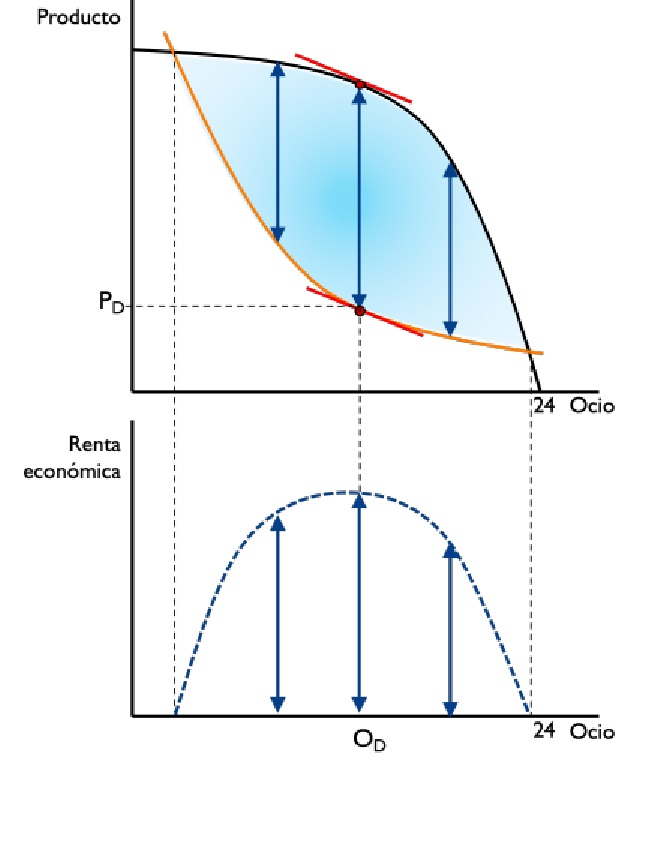
\includegraphics[scale=0.3]{Figures/Tema_04.9_modcap4_4.jpg}
\end{frame}

\begin{frame}
\frametitle{ ¿Qué pasa si el individuo puede decidir?}
\centering
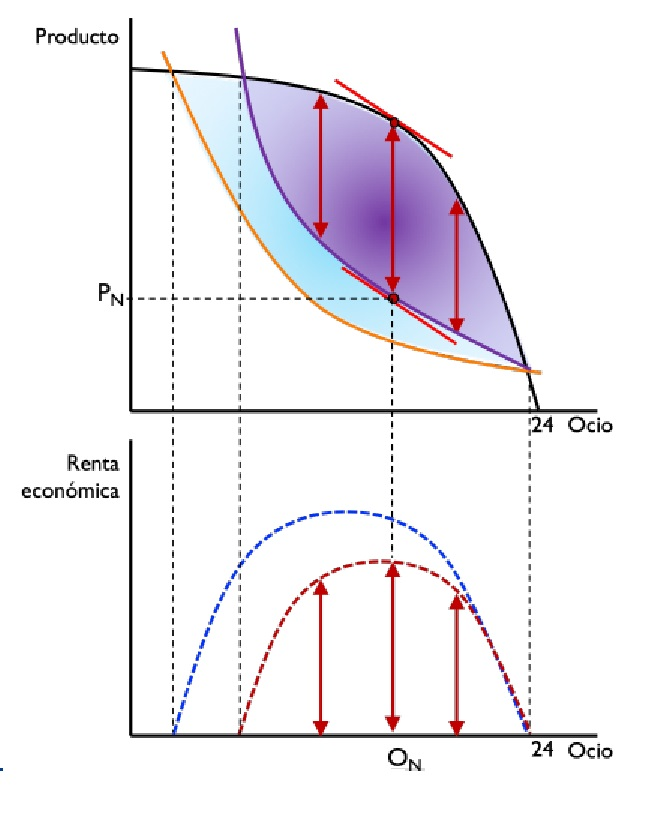
\includegraphics[scale=0.3]{Figures/Tema_04.11_modcap4_6.jpg}
\end{frame}

\begin{frame}
\frametitle{¿Qué pasa si sumo a los sindicatos?}
\centering
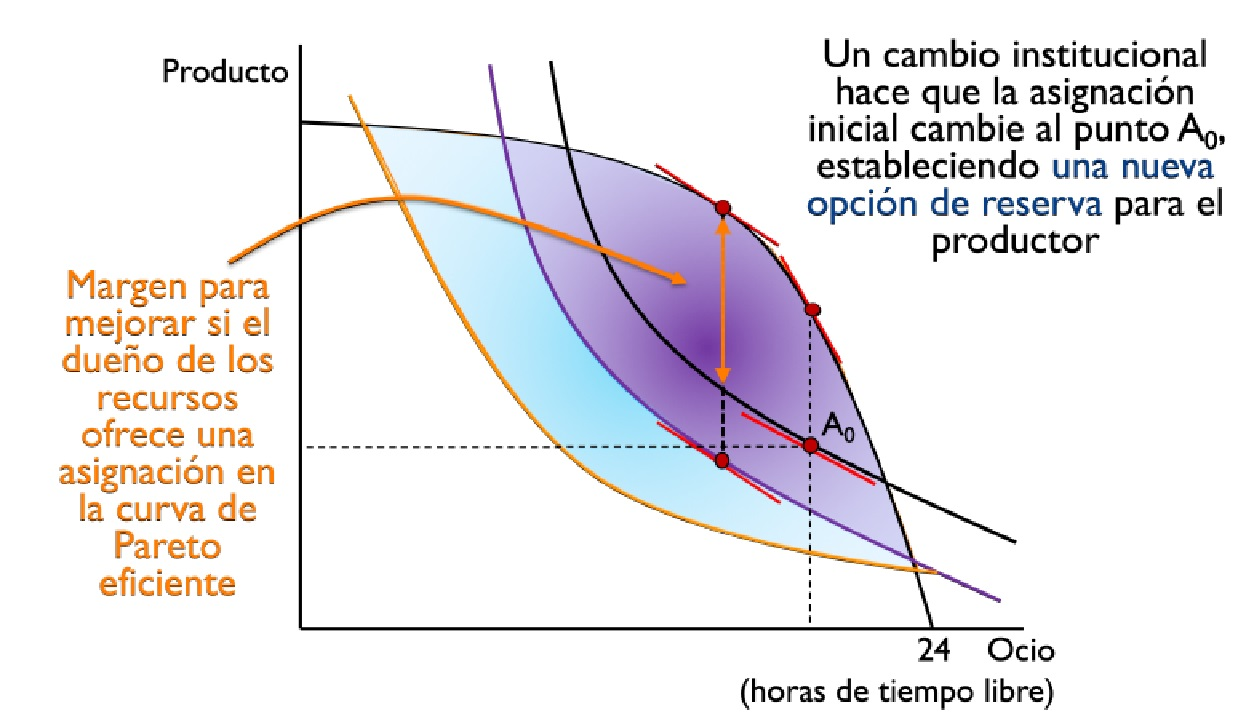
\includegraphics[scale=0.3]{Figures/Tema_04.13_modcap4_8.jpg}
\end{frame}

\begin{frame}
\frametitle{Factores que determinan una asignación}
\definecolor{Azul}{rgb}{0.1,0.1,0.6}
\begin{itemize}
    \item  \textcolor{Azul}{Instituciones}
    \item Tecnología
    \item Biología
    \item Preferencias
\end{itemize} 
\end{frame}

\begin{frame}
\frametitle{¿Qué es una institución?}
De acuerdo a North, las reglas del juego en una sociedad
    \begin{itemize}
    \item Que reducen la incertidumbre
    \begin{itemize}
        \item Y como consecuencia reducen los costos de transacción, proporcionando una estructura a la vida cotidiana
        \item Definen y limitan el conjunto de opciones de los individuos
    \end{itemize}
    \item Son creadas por seres humanos
        \begin{itemize}
        \item Normas formales e informales
        \end{itemize} 
    \item Afectan la performance de la economía
        \begin{itemize}
        \item Pueden inducir a aumentar o reducir la productividad
        \end{itemize} 
\end{itemize} 
\end{frame}

\begin{frame}
\frametitle{¿Qué es una institución?}
\begin{itemize}
    \item Greif [2006] dio una definición más precisa:
    \\ \vspace{2mm}
    ``Una institución es un sistema de reglas, creencias, normas y organizaciones que juntas generan una regularidad en la conducta''
    \\ \vspace{2mm}
    \item Una regularidad en el comportamiento social 
    \begin{itemize}
        \item Comportamiento en situaciones recurrentes...
        \item ... llevado a cabo por individuos que ocupan una posición social particular
    \end{itemize}
    \item Cada componente del sistema
    \begin{itemize}
        \item Es social al ser hecho por el hombre...
        \item ... y exógeno a cada individuo cuyo comportamiento influye
    \end{itemize}
\end{itemize} 
\end{frame}

\begin{frame}
\frametitle{Los componentes del sistema}
\begin{itemize}
    \item Las reglas, cuando son reconocidas socialmente, guían el comportamiento
    \begin{itemize}
        \item Crean un conocimiento compartido
        \item Proveen información y coordinan el comportamiento
        \item Indican el comportamiento socialmente aceptable
    \end{itemize}
    \item Las creencias y normas motivan a seguir reglas
    \begin{itemize}
        \item Normas y creencias internalizadas
    \end{itemize}
    \item Las organizaciones (formales o informales)
    \begin{itemize}
        \item Producen y difunden reglas
        \item Perpetúan creencias y normas
        \item Influyen en el conjunto de creencias factibles
    \end{itemize}
\end{itemize}
\end{frame}

\begin{frame}
\frametitle{ Discutamos ejemplos...}
\centering
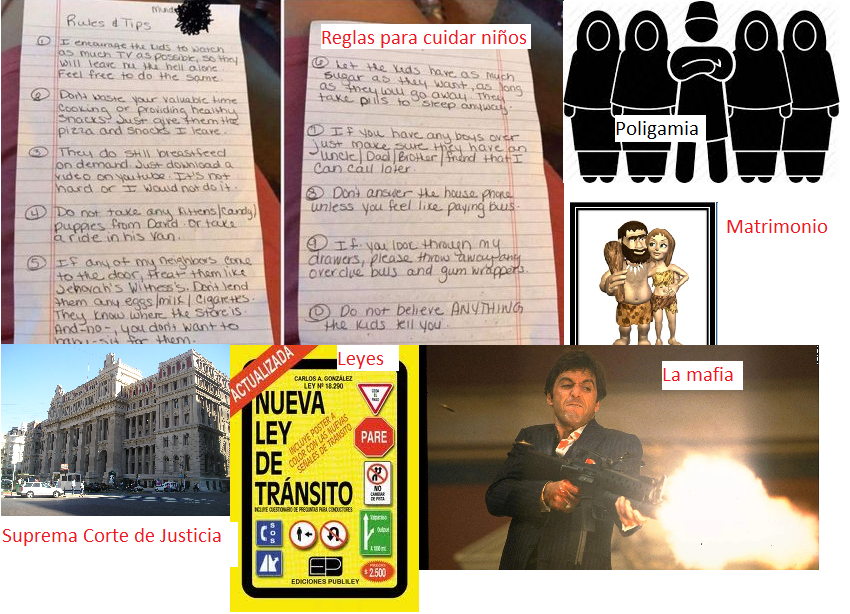
\includegraphics[scale=0.45]{Figures/Tema_04.1_examples.png}
\end{frame}

\begin{frame}
\frametitle{Importancia de las instituciones}
\begin{itemize}
    \item Al generar una regularidad en la conducta, las instituciones determinan qué tan grandes son los costos de transacción, y quien los paga
    \begin{itemize}
        \item Esto afecta si los agentes actúan o no
        \item Buenas instituciones reducen los costos de transacción, lo que implica más transacciones económicas
    \end{itemize}
    \item ¿Importan para el crecimiento?
\end{itemize}
\end{frame}

\begin{frame}
\frametitle{El problema de simultaneidad}
\centering
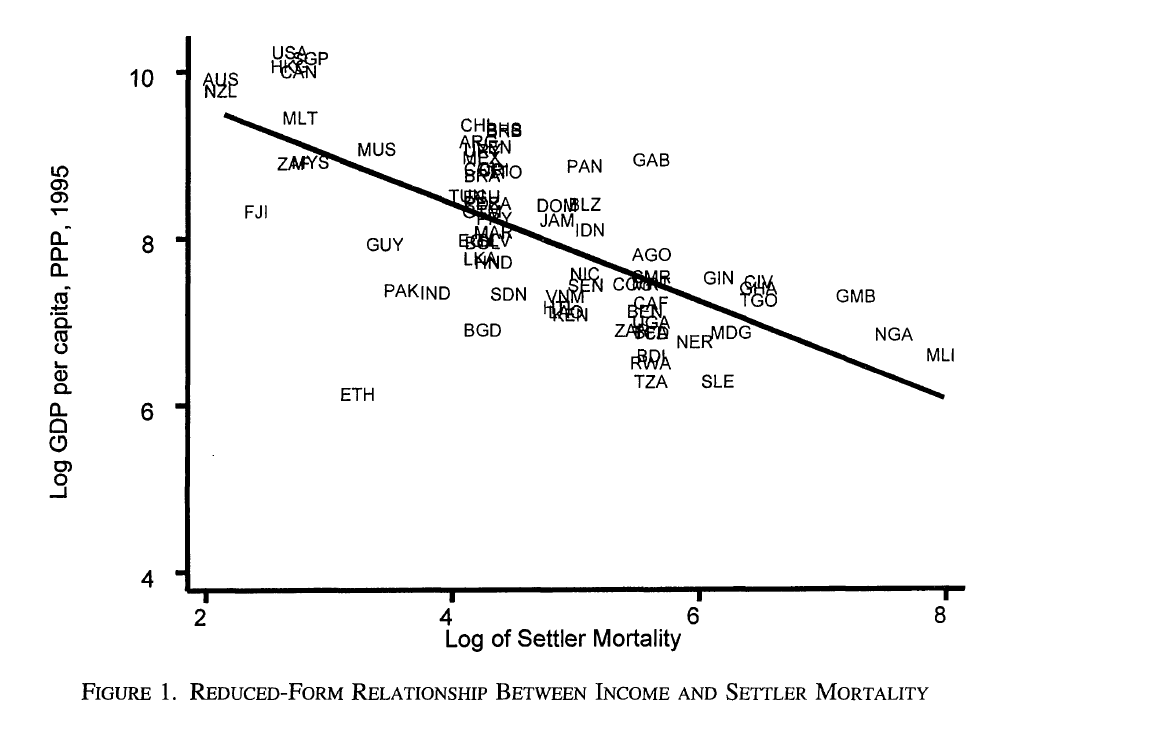
\includegraphics[scale=0.35]{Figures/Tema_04.1_examples2.png}
\small Fuente: Acemoglu, Johnson & Robinson (2001)
\end{frame}

\begin{frame}
\frametitle{ Asignaciones y justicia}
\begin{itemize}
    \item Una asignación puede ser considerada injusta por llegar a un resultado final desigual...
    \begin{itemize}
        \item Un juicio substantivo de la justicia \\
        - Para llevar a cabo este juicio necesitamos conocer básicamente el resultado para definir si es justo o no \\
        - Necesitamos una métrica de desigualdad en la asignación
    \end{itemize}
    \item ... pero puede también ser considerada injusta por la forma en que se llegó a ese resultado
    \begin{itemize}
        \item Un juicio procedimental de la justicia \\
        - Pare evaluar este aspecto, necesitamos entender las reglas de juego y cómo se llegó al resultado \\
        - ¿Fue el intercambio voluntario?, ¿Fueron algunos individuos discriminados?, etc.
    \end{itemize}
\end{itemize}
\end{frame}

\begin{frame}
\frametitle{ Economía y justicia}
\begin{itemize}
    \item Los valores que tiene la gente sobre lo que es justo y lo que no varía... ¿cómo lidiamos con cuestiones de justicia? ¿cómo ser imparcial en estos temas?
    \item El filósofo americano John Rawls sugirió hacerlo en tres etapas:
    \begin{itemize}
        \item Se adopta la idea que la justicia se aplica para todos
        \item El velo de la ignorancia: imaginarse detrás del velo de la ignorancia, es decir, imaginarse ocupando cualquier lugar posible en la sociedad que estamos considerando
        \item Elaboramos un juicio o evaluamos una institución desde atrás de ese velo
    \end{itemize}
\end{itemize}
\end{frame}

\begin{frame}
\frametitle{Economía y justicia}
\begin{itemize}
    \item La economía no puede proporcionar juicios sobre lo que es justo o no pero sí puede ayudarnos a pensar una serie de cosas: \vspace{2mm}
    \begin{itemize}
        \item Cómo las instituciones (reglas del juego) afectan la desigualdad
        \item Los trade-offs entre las distintas dimensiones de la justicia
        \item Qué tipo de políticas públicas pueden hacer frente a la injusticia
    \end{itemize}
\end{itemize}\end{frame}

\begin{frame} 
\frametitle{¿Cómo evaluamos una asignación?}
\begin{itemize}
\item Vimos que hay dos criterios para evaluar una asignación específica: 
\begin{itemize}
    \item Eficiencia
    \item Equidad
\end{itemize}
\item ¿Existe un trade off entre eficiencia y equidad?  \href{https://www.socialeurope.eu/good-bad-inequality}{No debería...}
\end{itemize}
\end{frame}
\end{document}


\begin{frame}
\frametitle{14. Curva Pareto eficiente}
\centering
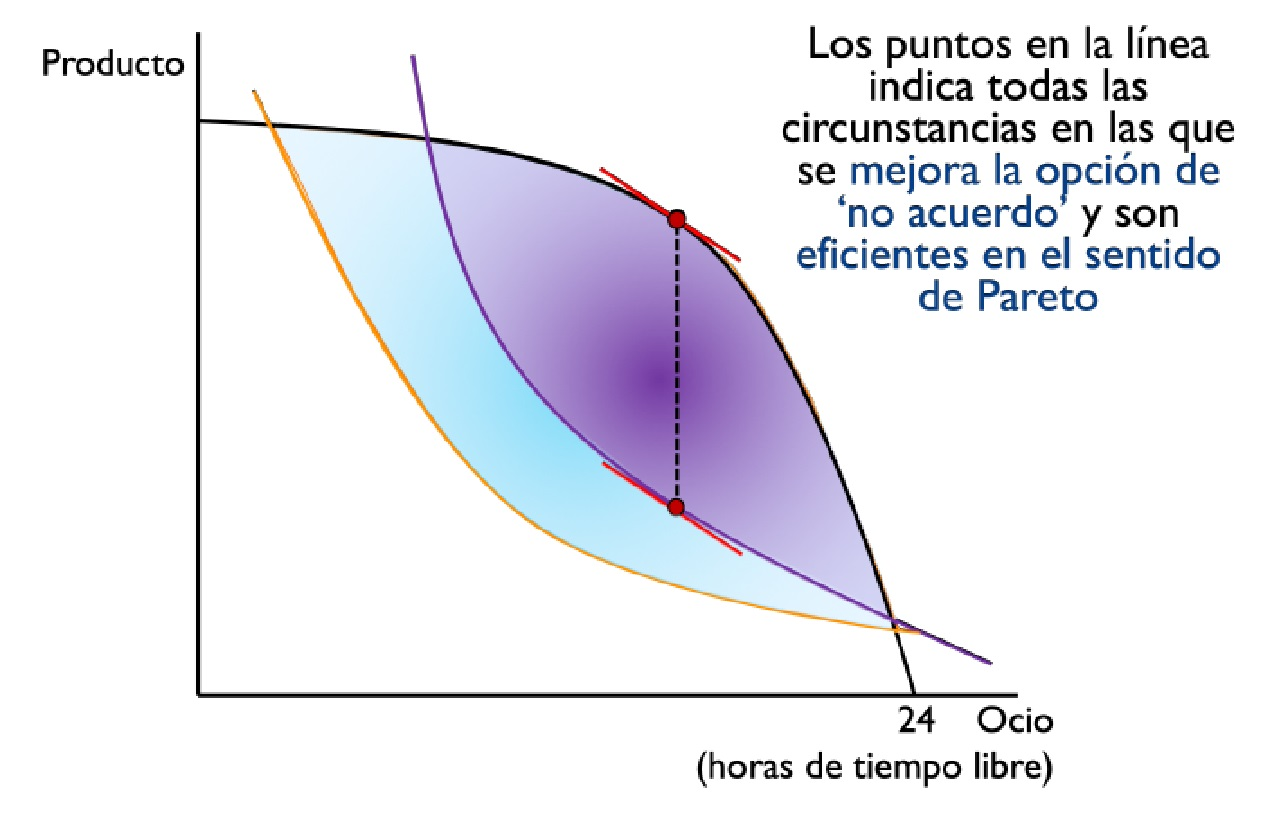
\includegraphics[scale=0.3]{Figures/Tema_04.12_modcap4_7.jpg}
\end{frame}




%%%%%%%%%%%%%%%%%%%%%%%%%%%%%%%%%%%%%%%%%%%%%%%%%%%%%%%%%%%%%%%%%%%%%%%%%
\begin{frame}
\frametitle{23. Juegos simultáneos}
\begin{itemize}
\item En los juegos simultáneos, cada jugador decide su estrategia antes de conocer las decisiones de otros jugadores
\item Para analizar estos juegos, usamos la matriz o forma estratégica de un juego
\item La combinación de las estrategias elegidas por los jugadores determina la ganancia de cada jugador
\end{itemize}
\end{frame}


\begin{frame}
\frametitle{25. Dilema del prisionero}
\begin{itemize}
\item Dos sospechosos son arrestados y acusados de un delito
\item La policía no tiene evidencia suficiente para condenar a los sospechosos a menos que uno confiese
\item La policía encierra a los sospechosos en celdas separadas y les explica las consecuencias derivadas de las decisiones que formen
\end{itemize}
\end{frame}

\begin{frame}
\frametitle{26. Dilema de los prisioneros}
\begin{itemize}
\item Si ninguno confiesa, ambos serán condenados por un delito menor sentenciados a un mes de cárcel
\item Si ambos, confiesan serán sentenciados a seis meses de cárcel
\item Finalmente, si uno confiesa y el otro no, el que confiesa será puesto en libertad inmediatamente y el otro
será sentenciado a nueve meses en prisión, seis por el delito y tres más por obstrucción a la justicia
\end{itemize}
\end{frame}

\begin{frame}
\frametitle{27. Dilema de los prisioneros}
\begin{table}
     \begin{tabular}{cc|c|c|}
      & \multicolumn{1}{c}{} & \multicolumn{2}{c}{Preso $2$}\\
      & \multicolumn{1}{c}{} & \multicolumn{1}{c}{No confesar}  & \multicolumn{1}{c}{Confesar} \\\cline{3-4}
      \multirow{}{Preso $1$}  & No Confesar & $(-1,-1)$ & $(-9,0)$ \\\cline{3-4}
      & Confesar & $(0,-9)$ & $(-6,-6)$ \\\cline{3-4}
    \end{tabular}
  \end{table}
\end{frame}

\begin{frame}
\frametitle{28. Dilema de los prisioneros}
\begin{itemize}
\item Cada jugador cuenta con dos estrategias posibles: confesar y no confesar. 
\item Las ganancias de los dos jugadores cuando eligen un par concreto de estrategias aparecen en la casilla correspondiente de la matriz binaria. 
\item Por convención, la ganancia del llamado jugador-fila (Preso 1) es la primera ganancia, seguida, por la ganancia del jugador columna (Preso 2). 
\end{itemize}
\end{frame}

\begin{frame}
\frametitle{29. Dilema de los prisioneros}
\begin{itemize}
\item Por ejemplo, el preso 1 elige no confesar y el preso 2 elige confesar, el preso 1 recibe una ganancia de -9 (que representa nueve meses en prisión) y el preso 2 recibe una ganancia de 0 (que representa la inmediata puesta en libertad).
\item La representación en forma normal de un juego especifica: 
\begin{enumerate}
\item [1] los jugadores en el juego,
\item [2] las estrategias de que dispone cada jugador, y 
\item [3] la ganancia de cada jugador en cada combinación posible de estrategias.
\end{enumerate}
\end{itemize}
\end{frame}







$$$$$$$$$$$$$$
\begin{frame}
\frametitle{22. Teoría de juegos y estrategia competitiva}
\begin{block}{Equilibrio de Nash}
Un equilibrio de Nash es un par de estrategias, una para cada jugador, en las que cada estrategia es la mejor respuesta dado lo que hace el otro
\end{block}
\vspace{5mm}
En equilibrio, cada jugador está haciendo lo mejor que puede, dado lo que el otro jugador también lo está haciendo
\end{frame}
$$$$$$$$$$$$$$$$$$

